%---Document Class---%
\documentclass[12pt]{report}

%---Packages---%
\usepackage[utf8]{inputenc} %Danish letters
\usepackage{authblk} %Title
\usepackage{graphicx}
\usepackage{sectsty}
\usepackage{caption}
\usepackage{subcaption}
\usepackage{listings}
\usepackage{setspace}
\usepackage{mathtools}  %Equations
\usepackage[usenames,dvipsnames]{xcolor}
\usepackage[hidelinks]{hyperref} %Emails in Title
\usepackage[toc,page]{appendix}
\usepackage{multicol}
\usepackage{pdfpages}

%---Colors---%
\definecolor{chapterColor}{HTML}{004685}
\definecolor{sectionColor}{HTML}{087D9C}
\definecolor{subSectionColor}{HTML}{07928A}
\definecolor{defaultColor}{HTML}{222222}

\chapterfont{\color{chapterColor}}
\sectionfont{\color{sectionColor}}
\subsectionfont{\color{subSectionColor}}
\color{defaultColor}

%---Fonts---%
%\usepackage{fontspec}
%\setmainfont{Arial}

\usepackage{iwona}
%\usepackage[default]{raleway}
%\usepackage{inconsolata}
\usepackage[T1]{fontenc}
\renewcommand\textbullet{\ensuremath{\bullet}}

%---Page Setup---%
\usepackage[a4paper, margin=2.5cm]{geometry}
\setlength{\parindent}{0em}
\setlength{\parskip}{1em}

\lstdefinestyle{customc}{
    belowcaptionskip=1\baselineskip,
    breaklines=true,
    xleftmargin=\parindent,
    language=C,
    showstringspaces=false,
    basicstyle=\footnotesize\ttfamily,
    keywordstyle=\bfseries\color{green!40!NavyBlue},
    commentstyle=\itshape\color{purple!40!NavyBlue},
    identifierstyle=\color{black},
    stringstyle=\color{orange},
    tabsize=4,
    numbers=left,
    numberstyle=\tiny\color{gray},
}

\lstset{style=customc}

%--- Bibliography ---%
\usepackage[backend=bibtex ,bibencoding=ascii]{biblatex}
\addbibresource{chapters/cha_bibliography/bibliography.bib}
\nocite{*}


%---Begin Document---%
\newcommand{\documentTitle}{Design, simulation and development of a bipedal locomotion platform for human-like gaits studies}
\newcommand{\documentType}{Master Thesis}

\newcommand{\institute}{University of Southern Denmark}
\newcommand{\department}{Faculty of Engineering}
\newcommand{\program}{MSc in Engineering, Robot Systems}
%\newcommand{\course}{Robot System Design}

\newcommand{\authorOne}{Jorge Rodriguez Marin}
\newcommand{\authorTwo}{Ignacio Torroba Balmori}

%---Begin Document---%
\begin{document}
    \pagenumbering{gobble} % Remove warnings of number page
	%!TEX root = ../../report.tex

% Title Page
\begin{titlepage}

	\begin{center}
	\includegraphics[width=60mm,keepaspectratio]{figures/sdu_logo}\\

	\vspace{0.3cm}
	\textbf{\institute}\\

	\textmd{\department}\\
	\textmd{\program}  %- \textmd{\course}
	\makebox[0pt][l]{
		\hspace{-14cm}
	  \raisebox{-\totalheight}[0pt][0pt]{
	  	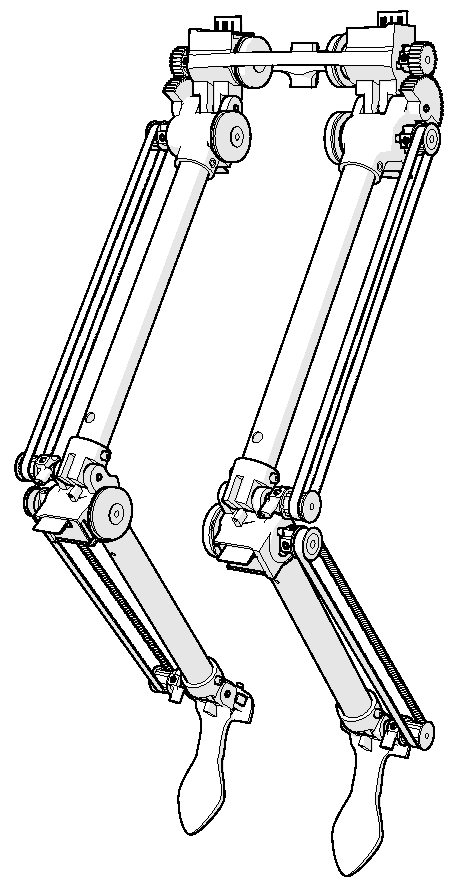
\includegraphics[height=180mm]{figures/legs_technical_drawing.pdf}
	  }
	% \makebox[0pt][l]{
	% 	\hspace{-20.5cm}
	%   \raisebox{-\totalheight}[0pt][0pt]{
	%   	\includegraphics[height=210mm]{figures/kittyParty.png}
	%   }
	}\\[4cm]

	\vspace{0.4cm}
	{\huge \bfseries \documentTitle}
	\\
	\vspace{0.5cm}
	{\large \documentType}
	\\[2cm]

	\begin{tabular}{c}
	 \makebox[4cm]{\emph{Authors}} \\
	 \makebox[4cm]{\authorOne} \\
	 \makebox[4cm]{\authorTwo} \\
	\end{tabular}

	\vfill
	{\large \today}
	\end{center}

\end{titlepage}

    \pagenumbering{arabic} % Remove warnings of number page
    \setcounter{page}{2}

    %\tableofcontents\thispagestyle{empty}\vfill % No number page
    %\onehalfspacing
    \singlespacing
	\tableofcontents
    \listoftables
    \listoffigures

    %!TEX root = ../report.tex
\chapter{Introduction}
\label{chap:introduction}

\section{Overall description}
The goal of this project is 

\subsection{Report structure}
The report is organized so it starts with	
    %!TEX root = ../../report.tex
\chapter{State of the art} % (fold)
\label{cha:state_of_the_art}
%!TEX root = ../../../report.tex
\section{Motivation} % (fold)
\label{sec:sim_motivation}
What is a simulator, why to simulate

% section motivation (end)
%%!TEX root = ../../report.tex
\chapter{State of the art} % (fold)
\label{cha:state_of_the_art}
%!TEX root = ../../../report.tex
\section{Motivation} % (fold)
\label{sec:sim_motivation}
What is a simulator, why to simulate

% section motivation (end)
%%!TEX root = ../../report.tex
\chapter{State of the art} % (fold)
\label{cha:state_of_the_art}
\input{chapters/cha_state_of_the_art/Sections/sec_motivation}
%\input{chapters/cha_state_of_the_art/cha_state_of_the_art}
\input{chapters/cha_state_of_the_art/Sections/sec_theoretical_background}
%\section{Theoretical background}

%\section{Current research}
% chapter state_of_the_art (end)
%!TEX root = ../../../report.tex

\section{Theoretical background}
\label{sec_theoretical_background}



Difficulties to calculate compliance added by springs configuration for specific applications.
Possibility to change the springs configurations
Study of adaption of neural controllers to robot platforms whose mathematical model is hard to define due to added compliance.
Possibility of comparing controllers performance in two different platforms

%\section{Theoretical background}

%\section{Current research}
% chapter state_of_the_art (end)
%!TEX root = ../../../report.tex

\section{Theoretical background}
\label{sec_theoretical_background}



Difficulties to calculate compliance added by springs configuration for specific applications.
Possibility to change the springs configurations
Study of adaption of neural controllers to robot platforms whose mathematical model is hard to define due to added compliance.
Possibility of comparing controllers performance in two different platforms

%\section{Theoretical background}

%\section{Current research}
% chapter state_of_the_art (end)
    %!TEX root = ../../report.tex
\chapter{Analysis} % (fold)
\label{cha:analysis}
The process of designing and constructing a bipedal robot as the presented here is a task of great magnitude in which a big set of parameters has to be analyzed and determined aiming at the most optimal solution possible. \footnote{Optimality here is measured in terms of the aimed goals, described in \ref{sec:goals}.}
Thus, the sections in this chapter contain the conceptual analyses conducted as the initial step in the conception of the RuBi prototype, together with a summary presentation of the research done in human locomotion 
Its results will be used as guidelines for the posterior and more detailed studies carried out during the implementation of the robot.

%!TEX root= ../../../report.tex

\section{Bipedal locomotion} % (fold)
\label{sec:bipedal_walking_and_running_gaits}

%General presentation of concepts and definitions
%Froud number computed
%Requirements for walking and running


% section bipedal_walking_and_running_gaits (end)
%!TEX root = ../../../report.tex

\section{Geometrical dimensions of the frame} % (fold)
\label{sec:dimensions}

The selection of the final dimensions of RuBi corresponds to an iterative process in which power requirements have been the first constraint when assessing the size of the robot.
A first approach was taken from \cite{grimmer}, Manuscript I, where normalized values of power required per joint and per kilogram of the structure can be found.
The first iteration targeted a robot of dimensions $m = 1Kg$ and length from the hip joint to the tip toes of $L = 0.6 m$ for a fully stretched leg.
The final parameters from the last iteration can be found in ***%***chapter Results

Once estimated an overall length of the structure, the dimensions of each link were decided to be obtained based on the German section of the ISO 7250-2 \cite{iso_measurements} and the DIN 33402-2 \cite{din_measurements1} norms, following the idea of mimicking human-like motion as closely as possible.
These two norms are standard references in industry and were considered a general enough source of information.
Figure \ref{fig:human_measurements} depicts some of the human dimensions extracted from the norms and applied to the design of RuBi.
Their names and values for male between 18-65 year old and in percentile 50 can be found in table \ref{tab:din_proportions}.

\begin{figure}[h]
	\centering
	\begin{subfigure}[b]{0.3\textwidth}
        \includegraphics[width=\textwidth]{figures/din_measurements.pdf}
        \caption{Left foot}
        \label{fig:din1}
    \end{subfigure}
    \begin{subfigure}[b]{0.4\textwidth}
        \includegraphics[width=\textwidth]{figures/din_measurements2.pdf}
        \caption{Hip}
        \label{fig:din2}
    \end{subfigure}
	\caption{Lower body measurements used for RuBi. Picture adapted from \cite{din_measurements1}.}
	\label{fig:human_measurements}
\end{figure}


\begin{table}
\begin{center}
	\begin{tabular}{c | c | c | c}
	  Index & Definition & Value & \% of Stature \\
	  \hline
	  A & Stature (body height) & ** & 100 \\
	  B & Crotch height & ** & ** \\
	  C & Femur height & ** & ** \\
	  D & Tibial height & Not in norm & **\\
	  E & Ankle-toe tip distance & Not in norm & ** \\
	  F & Buttocks-leg length & ** & ** \\
	  G & Sole length & ** & **
	\end{tabular}
	\caption{Human proportions from DIN 33402-2}
	\label{tab:din_proportions}
\end{center}
\end{table}

The dimensions needed to create a simplified model of one leg are the limbs lengths, which are the straight line distances measured from two consecutive joints.
They have been called $L_{i}$ where $i$ is the robot link + joint as per table \ref{tab:limb_index} and can be seen in Figure \ref{fig:kinematics}.
However, the norm does not determine all of them.

\begin{table}
\begin{center}
	\begin{tabular}{c | c | c}
	  $L_{i}$ & Limb \\
	  \hline
	  $L_{1}$ & Hip + thigh & C \\
	  $L_{2}$ & Knee + Foreleg & D\\
	  $L_{3}$ & Ankle + foot & E 
	\end{tabular}
	\caption{Limbs index}
	\label{tab:limb_index}
\end{center}
\end{table}

Since $C$ and $E$ are not standard measurements in industry, they have been obtained as follows:

\paragraph{The Femur height}
The crotch height, denoted as $B$ in the figure, has been averaged with the buttocks-leg length and the tibial height + an empirical approximation of the height of the ankle have been subtracted from the result, obtaining $C$.

\paragraph{The ankle-toe tip distance}
Since this distance is not standard either, it has been obtained once again adjusting the sole length with empirical measurements.

%% Here we just describe the process followed to obtain the final dimensions. 
%% The final results are shown in Chapter Results --> add tables and Froude number calculus


% section dimensions (end)
%!TEX root = ../../../report.tex

\section{Physical properties} % (fold)
\label{sec:physical_properties}

% section physical_properties (end)
%!TEX root = ../../../report.tex
\section{Joints} % (fold)
\label{sec:joints}
Following the idea of mimicking the human lower-body structure it was decided to implement three actuated rotational joints per leg although some research was conducted on the use of passive ankles as in \cite{dacbot1}, \cite{phides} or \cite{mabel}.
However, the results introduced in \cite{grimmer} from their analysis of joint actuation for prosthetics limbs proved the importance of the actuation in the ankles for running.

The design of the joints entailed the addressing of three main areas

\begin{itemize}
  \item Actuator model
  \item Transmission system
  \item Implementation of dedicated compliance
\end{itemize}

% \begin{figure}[ht!]
%   \centering
%   \includegraphics[width=\textwidth]{figures/20160518_195014.jpg}
%   \caption{Might help}
%   \label{fig:figure1}
% \end{figure}

\subsection{Actuators} % (fold)
\label{sub:actuators}
In humans, the actuation of the joints is mostly provided by pairs of agonist-antagonist skeletal muscles linked to the bones through the tendons \cite{anatomy}.
The activation-inhibition of these muscles produce a lever effect on the bones that leads to its control and motion by modifying the angle between two consecutive limbs.
To achieve the same kind of motion control, the implementation of a similar system through electric linear actuators was considered.
However, the time constraints, their price and their complexity led to discard them and select conventional electric motors.
The selected motor model will have to be able to provide a sufficient torque to generate the desired forces at the end of the link, following equation \ref{eq:torque}.

\begin{equation}
\label{eq:torque}
  \tau = r \times F
\end{equation}

This equation could be sufficient to compute the torque required by the load for a motor application of leverage. 
However, an study of each joint separately would not provide an accurate enough solution due to the configuration of the legs, making necessary an study of the actuation as for a kinematic chain.
The analysis of the actuators requirements is to be found in \ref{cha:mathematical_model}.

% subsection actuators (end)

\subsection{Transmission} % (fold)
\label{sub:transmission}
As introduced in \ref{sub:moments_of_inertia}, the reduction of the moments of inertia in the limbs in order to minimize the torque requirements for motion was set as a priority.
This led to the study of methods to displace the CoM of the limbs as close to their joints axes as possible, thus reducing their inertias.
The solution was to place the actuators, the heaviest components of the design, as close to the upper part of the frame as possible, which would also result in the allocation of the CoM of the frame upper in the sagital plane.
An schematic example of this idea can be seen in the Figures in \ref{fig:compliance} for the ankle actuation, where the motor has been placed under the knee axis. 
The same principle has been applied to the knee actuation, as can be seen in the final implementation. 
For the hip, however, it was not necessary to install a transmission system, but a gear mechanism whose justification is to be found in \ref{cha:mathematical_model}.

Due to the new arrangement, a powertrain was required to transmit the torque to the joints.
It was decided to implement a system of 2 pulleys + belt due to its simplicity and optimal capabilities for the project requirements.
The goal of this mechanism is only the transmission of power, without any further adjustment of angular speed-torque ratios.
The calculations to find the optimal dimensions of the system are contained in \ref{sub:pulleys_and_belts}.
The pitfall of this implementation, however, is the introduction of delays in the motion transmission and the natural loss of accuracy arisen from the backlash associated to the use of pulleys.
Modeling these uncertainties for a classic locomotion controller based on the motion equations is proved a complex task. 
However it was assumed here that the ANN controllers that would drive the RuBi platform would be able to adapt to them without a model of the robot.

%Reduction of the moments of inertia
%Introduction of delays and loss of accuracy 

% subsection transmission (end)

\subsection{Compliance} % (fold)
\label{sub:compliance}

%Flexible vs stiff drive train
%Power peak and average consumption comparisons --> energy storage 
%Protection against impact forces on landing phase


\begin{figure}[hb!]
\label{fig:compliance}
  \begin{subfigure}{.19\textwidth}
    \centering
    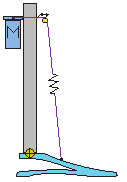
\includegraphics[width=\linewidth]{figures/illustration_serial_pulley.pdf}
    \caption{Serial pulley}
    \label{fig:series_pulley}
  \end{subfigure}
  \begin{subfigure}{.19\textwidth}
    \centering
    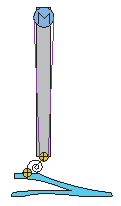
\includegraphics[width=\linewidth]{figures/illustration_serial_rotational.pdf}
    \caption{Series rotational}
    \label{fig:series_rotational}
  \end{subfigure}
  \begin{subfigure}{.19\textwidth}
    \centering
    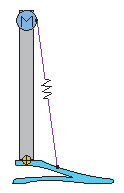
\includegraphics[width=\linewidth]{figures/illustration_serial_direct_i.pdf}
    \caption{Series direct 1}
    \label{fig:series_direct_i}
  \end{subfigure}
  \begin{subfigure}{.19\textwidth}
    \centering
    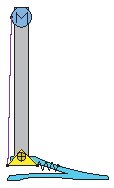
\includegraphics[width=\linewidth]{figures/illustration_serial_direct_ii.pdf}
    \caption{Series direct 2}
    \label{fig:series_direct_ii}
  \end{subfigure}
  \begin{subfigure}{.19\textwidth}
    \centering
    \includegraphics[width=\linewidth]{figures/illustration_serial_elastic_band.pdf}
    \caption{Series elastic band}
    \label{fig:series_elastic_band}
  \end{subfigure}
\end{figure}  

% subsection compliance (end)

% section joints (end)

% chapter analysis (end)
    %!TEX root = ../../report.tex
\chapter{Kinematic and dynamic model} % (fold)
\label{cha:kinematic_and_dynamic_model}

\section{Kinematic model}
\label{sec_kinematic_model}
%!TEX root= ../../../report.tex
\section{Dynamic model}
\label{sec_dynamic_model}
The goal of this step is to calculate the relationship between an external force applied to the toe (ground reaction force while jumping) and the necessary torques in the joints for dealing with that external disruption.
This relation can be expressed as a set of second order differential equations represented for the general case as in equation \ref{eq:dynamics_eq1}. 
\begin{equation}
	\label{eq:dynamics_eq1}
	B(q)\ddot{q} + C(q,\dot{q})\dot{q} + g(q) = \tau
\end{equation}
Where $B(q)$ is the inertia matrix, $c(q,\dot{q})$ contains the centrifugal and coriolis acceleration terms and $g(q)$ represents gravity, as in \cite{dynamics1} and \cite{dynamics2}. 
It must be remarked here that the constructed model does not introduce joint friction terms.
For an open kinematic chain as this, three methodologies to obtain the above equation where object of study:
\begin{itemize}
	\item A simplified Euler-Lagrange algorithm, as introduced in \cite{E-L1}, which makes use of the Lagrangian formulation to describe the behavior of the system through work and energy.
	\item The so called Energy Method, presented in \cite{asada} and consisting in finding the relation between the force in the end-effector and the joint torques through the Jacobian of the kinematic chain.
	\item The Newton-Euler algorithm, through which the dynamics of the system can be expressed in terms of forces and moments applied in each member of the chain.
\end{itemize}
It was finally decided to apply the third option due to the fact that it was faster to implement than the E-L algorithm and more reliable than the Energy method.
The Newton-Euler algorithm is founded in classical mechanics and its a recursive method that computes in two steps the velocities and accelerations of every component of a kinematic chain and their forces and torques on the joints.
In \ref{eq:N-E_eq1}, the equations of motion for an individual link are shown.
\begin{equation}
\label{eq:N-E_eq1}
	\begin{aligned}
		f_{i-1, i} - f_{i,i+1} + m_{i} g - m{i} \dot{V}_{ci} =& 0 \\
		N_{i - 1 , i} - N_{i , i + 1} - ( r_{i - 1 , i} + r_{i , Ci} ) \times f_{i - 1 , i} + ( - r_{i , Ci} ) \times ( - f_{i , i + 1}) - I_{i} \dot{\omega_{i}} - \omega_{i} \times ( I_{i} \omega_{i} ) =& 0 \\
		i = 1,..., N 
	\end{aligned}
\end{equation}
These equations contain the coupling forces and moments applied to the link by the immediate ones, however, they cannot be used with them. 
$\omega_{i}$ and $\dot{\omega_{i}}$ represent respectively the angular velocity and acceleration vectors of link $i$ and can be obtained from the joint velocities and accelerations, computed in the previous section, as in equation \ref{eq:angular_magnitudes}.
$I_{i}$ are the inertia matrices of the links, calculated in SolidWorks for the final design of RuBi.
\begin{equation}
\label{eq:angular_magnitudes}	
	\begin{aligned}
		\omega_{i} &= \omega_{i-1} + \xi_{i}\dot{q}_{i}Z_{base}^i\\
		\dot{\omega_{i}} &= \dot{\omega_{i-1}} + \xi_{i}[\ddot{q}_{i}Z_{base}^i + \dot{q}_{i}\omega_{i-1} \times Z_{base}^i]
	\end{aligned}
\end{equation}
The closed-form equations must be derived from them so that they can be applied to the algorithm.
This is done by substituting the coupling forces in the final set of 6 equations obtained for $N=3$ and substituting \ref{eq:torques} in the resulting equations.
\begin{equation}
\label{eq:torques}
	N_{i - 1 , i} = \tau_{i}
\end{equation}
Equation \ref{eq:torques} is valid only for the planar case.
After these steps, a set of three equations of the form \ref{eq:dynamics_eq1} is obtained. 
As parameters, they contain the masses of the links, their vectorial positions, the gravity term and their inertia matrices. 

This set of equations calculates the necessary torques on the joints as a function of the joints displacements and the external forces and torques applied on the system, as represented in \ref{eq:tau_q}.
\begin{equation}
\label{eq:tau_q}
	\tau(t)_{i} = f(q_{i}(t), \dot{q}_{i}(t), \ddot{q}_{i}(t), \tau_{ext}, F_{ext})
\end{equation}
However, in order to use it the functions that model the trajectories of joints in the joint space must be approximated.
For the ideal static, vertical jump case under study here, the movement of the toe has been constrained to a vertical displacement along the $Y$ axis in order to simplify this task.
Thus, the trajectory of the end-effector of the kinematic chain, $P_{3}$ in Figure \ref{fig:f-t}, can be easily approximated as a function of the form shown in 
\begin{equation}
\label{eq:toe_trajectory}
	\begin{aligned}
	x_{3}(t) &= 0 \\
	y_{3}(t) &= y_{3}(t_{o}) + \cfrac{y_{3}(t_{f}) - y_{3}(t_{o})}{(t_{f} - t_{o}) (t - t_{o})} \\
    \theta(t) &= \theta(t_{o}) + \cfrac{\theta(t_{f}) - \theta(t_{o})}{(t_{f} - t_{o}) (t - t_{o})} 
    \end{aligned}
\end{equation}
Therefore, if equation \ref{eq:toe_trajectory} is used as the input to the inverse kinematic model, the joint displacements will become dependent on the linear displacement of $P_{3}$, and equations \ref{eq:tau_q} will be rewritten as \ref{eq:tau_p}.
\begin{equation}
\label{eq:tau_p}
	\tau(t)_{i} = f(P_{3}(t), \tau_{ext}, F_{ext})
\end{equation}
\section{Actuators}
\label{sec_actuators}
%!TEX root= ../../../report.tex

\section{Springs}
\label{sec_springs}
%Furthermore, all the studies conducted in the influence of compliance in legged locomotion have been carried out over empirical data recorded for the specific task under analysis.
%All the studies found to optimize the value of springs focus only in a specific velocity and pattern --> we want a wide range of speed and both walk and run

%!TEX root= ../../../report.tex

\section{Model-based controllers}
\label{sec_dynamic_controller}
As introduced in the previous sections, the equations of motion derived for RuBi can be used to compute the necessary output values of its actuators in order to perform an input toes trajectory and external forces, as expressed in \ref{eq:tau_p}.
By definition, this could be sufficient to, appropriately used, be utilized as the base of a controller for the robot, without accounting the own dynamics of the actuators.
As an example of the above said, and despite the early stage in its development in which this model is left, some data has been computed and plotted for proving the concept.
The only trajectory planner current implemented computes vertical straight paths for the toes.
However, more complex trajectory equations could be used to achieve different locomotion patterns.

\begin{figure}[htb]
	\centering
	\includegraphics[width=0.5\textwidth]{figures/kinematics_sim.pdf}
	\caption{Joints trajectories from kinematics model.}
	\label{fig:controller_position}
\end{figure}

An initial and final toes position has been inputed to \ref{eq:toe_trajectory} to define an example trajectory for the toes in one leg, together with a random value for $\Delta h$.
The output of the kinematics computed for $i=1,...,N$ steps is shown in Figure \ref{fig:controller_position}, where it has been rearranged for visualization.
It can be seen that the toes trajectory does not cover the full range of a vertical jump.

\begin{equation}
\label{eq:joint_vel}
	\dot{\theta}_{i,j} =\frac{ \abs{ \theta_{j}(t_{i}) - \theta_{j}(t_{i-1}) } }{ t_{step} }
\end{equation}

For the trajectory described and $\Delta h$, the impulse equation in \ref{eq:impulse} has been computed and the values $(F_{min}, t_{max})$ from \ref{eq:work} have been used as input to the dynamic model.
The result of computing \ref{eq:dynamics_eq1} for the same time steps is shown in \ref{fig:controller_torque}, together with the solution for equation \ref{eq:joint_vel} in \ref{fig:controller_speed}, calculated in an analogue way.

\begin{figure}[htb]
    \centering
    \begin{subfigure}{0.49\textwidth}
        \includegraphics[width=\textwidth]{figures/torque-time.pdf}
		\caption{Joints torque as a function of time.}
		\label{fig:controller_torque}
	\end{subfigure}	
    \begin{subfigure}{0.49\textwidth}
        \includegraphics[width=\textwidth]{figures/speed-time.pdf}
		\caption{Joints velocity as a function of time.}
		\label{fig:controller_speed}
    \end{subfigure}
    \caption{Joint torque and velocity as a function of time.}
\end{figure}

The ranges in which the results in \ref{fig:controller_torque} and \ref{fig:controller_speed} are found seem consistent with the obtained during the experiments detailed in \ref{sub:suitability_of_the_motor_model_for_the_application}.
However, the analysis of their accuracy would entail a more precise construction of the mathematical model and study of kinematic chains dynamics which laid out of the scope of this project since it was not considered a priority goal.


% chapter kinematic_and_dynamic_model (end)
    %!TEX root = ../../report.tex
\chapter{Mechatronic design} % (fold)
\label{cha:design}
The results of the conceptual studies conducted in chapter \ref{cha:analysis} laid the goals and criteria to lead the design process of the first prototype of RuBi.
The actual implementation of these ideas in the fields of electronics, mechanics and software is described here.
When designing from a holistic point of view, these three areas combined give a positive synergy which is the burden of this chapter.
The first of the three sections starts with the design of the electronic hardware: from the selection of the motors based on \ref{sec:joints} and \ref{cha:mathematical_model} to the expansion interfaces installed in order to reduce the weight and finally the sensory feedback system.
It follows the mechanical design of the limbs components, in which the constraints defined in \ref{sec:dimensions} and \ref{sec:physical_properties} are applied, together with the structural and production-oriented calculations required.
It concludes with a presentation of the CAD design process carried out, in which a comprise between the components ideal capabilities and the current production capacity in this project has been tried to be reached.
In the last section, devoted to the software-related development except for the simulation environment, the architecture implemented for the robot control system is presented.

%!TEX root = ../../../report.tex
\section{Electronics} % (fold)
\label{sec:electronics}

%!TEX root = ../../../../report.tex

\subsection{The electric actuators} % (fold)
\label{sub:electric_actuators}
In chapter \ref{cha:mathematical_model}, the necessary characteristics of the actuators have been calculated.
In this section, the resulting theoretical requirements are used to select the final motor $+$ gearbox combination utilized.
All the documentation regarding the control of the actuators software-wise is to be found in section \ref{sec:software}.

\subsubsection{Flat BLDC Maxon motors} % (fold)
\label{ssub:the_bldc_motors}
It must be mentioned at this point that the actuators and their interface were assumed at the beginning of the project to be a very hard constraint in the design from an economic point of view. 
This means that the conception of the robot structure has been influenced by this criteria towards the adaption of the final prototype characteristics (such as final size or mass) to the application range of the available motors at our disposal.
This fact has converted the design in an iterative process of optimization whose final result is a robot that matches the available actuators and not the other way around, as it should be in theory.
In the view of the this, the brushless DC motor $+$ gearbox present in the Locokit robot construction kit, introduced in \cite{locokit} are used in the RuBi prototype.

The flat motors model is 339260 from Maxon motor, whose datasheet can be found in \cite{maxon_motor}, and the planetary gearhead is the number 143976 in datasheet \cite{maxon_gear}.
The electromechanical constants of the motors, together with its nominal supply values or the output power and torque of both the motor and the gearbox can be found in these documents. 
However, the electronics of the motors are designed to constantly overdrive them at $24V$, which has been taken into account when calculating their output.
Furthermore, each motor counts three hall effect sensors able to provide accurate relative position measurements.
% subsubsection the_bldc_motors (end)


\subsubsection{BLDC motor boards} % (fold)
\label{ssub:bldc_motor_boards}
Each BLDC motor in the Locokit comes with a motor board able to control it, designed for 24V and 48W.
They consist of a 48MHz ARM7 processor for time critical control and motor commutation, as stated in \cite{locokit-electronics}, together with 4 general purpose I/O inputs for local sensor interface.
Furthermore, they have two available 8-pin interfaces for the motors, one of them with a standard flex connector used in most of Maxon flat motors.

% subsubsection bldc_motor_boards (end)

\subsubsection{Extension PCBs} % (fold)
\label{ssub:extension_pcbs}
Following the idea of reducing weight and inertias in the structure as explained in chapter \ref{cha:analysis}, it was decided to place all the electronics off-board.
In order to extend the existing motor flex interfaces, a simple extension PCB was manufactured for each device.
The boards have been designed with Eagle following the requirements of current when sizing the width of the paths given by the supplier.
The design lacks of vias which reduces the complexity and facilitates the manufacturing.
The board for the left leg, whose schematic can be seen in \ref{fig:pcb1}\footnote{For the right leg the schematic has been mirrored}, contains a flex connector, like the one originally found on the motor boards, mapped to an 8-pin Molex connector where the wiring to the BLDC board is connected.

\begin{figure}[ht]
	\centering
	\includegraphics[width=0.5\textwidth]{figures/expansion_board.pdf}
	\caption{Left leg extension PCB schematic.}
	\label{fig:pcb1}
\end{figure}

% subsubsection extension_pcbs (end)


% subsection electric_actuators (end)
\subsection{Suitability of the motor model for the application} % (fold)
\label{sub:suitability_of_the_motor_model_for_the_application}
The algorithm designed to prove if the selected motor model fulfills the requirements of the application has been called Algorithm 1 and it is detailed in \ref{list:algorithm_1}.
The theoretical framework constructed in \ref{cha:mathematical_model} has been applied here to prove if the motors described above (without accounting on springs or indirect transmission) can be used to perform the vertical jumps described in \ref{sec:jumping_case}.
And if so, which height can be reached.

Algorithm 1:
\begin{enumerate}
\label{list:algorithm_1}
\item Manually set the values of $P_{3}(t_{0})$ and $P_{3}(t_{f})$ to use in equation \ref{eq:toe_trajectory}.
\item Compute the inverse kinematics model for the given trajectory equation. This yields as outputs $q_{j}(t)$, where j = 1,...,N being N = number of joints.
\item Compute forward kinematics to obtain $P_{j}(t)$.
\item Derive the two mentioned models and apply equation \ref{eq:angular_magnitudes} to obtain $\dot{P}_{j}$, $\ddot{P}_{j}$, $\omega_{j}$, $\omega_{j}$, $\dot{\omega}_{j}$,
\item Set $\Delta h$ and use the impulse equations \ref{eq:deltaV} and \ref{eq:impulse} to obtain a set of couple values of $(F_{i}, t_{i})$ as in Figure \ref{fig:f-t}.
\item For each couple until $(F_{min}, t_{max})$, obtained from \ref{eq:work}, compute the torques $\tau_{i,j}$ for each joint through \ref{eq:dynamics_eq1} and $\theta_{i,j}$ as in \ref{eq:joint_vel_2}\footnote{Eq. \ref{eq:joint_vel_2} introduced the assumption that the joint velocities are constant for simplicity}.
\item Compute the Torque/Speed curve for the motor + gearbox model as per equation \ref{eq:motor_curve}.
\item Plot the obtained pairs of values $(\dot{\theta}_{i,j}, \tau_{i,j})$ over the motor curve and analyze the results.
\end{enumerate}

\begin{equation}
\label{eq:joint_vel_2}
	\dot{\theta}_{i,j} =\frac{ \abs{ \theta_{j}(t_{f}) - \theta_{j}(t_{o}) } }{ t_{i} }
\end{equation}

\begin{equation}
\label{eq:motor_curve}
	\tau_{m} = \tau_{stall} - \omega_{m}\left(\frac{\tau_{stall}}{\omega_{n}}\right)
\end{equation}

\paragraph{Use case} % (fold)
\label{par:example_of_use}
As with any kind of DC motor, the goal is that the operation points lay under the torque/speed curve for a given application.
In this case, the operation point to study has been chosen to be the initial instant of the launch phase during the jump, given by $t_{0}=0s$, because it has been assumed to be the most requiring one of the whole jump cycle.
The input data for the test conducted with the algorithm can be seen in \ref{eq:input_a1}.

\begin{equation*}
\label{eq:input_a1}
\begin{aligned}[c]
P_{3}(t_{0}) &= \left[\!
				    \begin{array}{c}
				      0 \\
				      0.3508 \\
				      -\frac{\pi}{2}
				    \end{array}
				  \!\right]
\end{aligned}
\qquad
\begin{aligned}[c]
P_{3}(t_{f}) &= \left[\!
				    \begin{array}{c}
				      0 \\
				      L \\
				      0
				    \end{array}
				  \!\right]
\end{aligned}
\qquad
\begin{aligned}[c]
\Delta h &= 0.05 \\
\end{aligned}
\end{equation*}

The results can be seen in Figure \ref{fig:alg1_results} for a jumping leg.
It can be seen that, for the obtained $(\theta_{i,j}, \tau_{i,j})$ values for the given $\Delta h$, the closer they get to the theoretical $(F_{min}, t_{max})$, the more the application points approach the lower-left corner of the graph.
The aimed situation here is that in which the application points for the three motors lay under the motor curve, which occurs for values next to the couple $(4.1191N, 0.1700s)$

\begin{figure}[htb]
	\centering
	\includegraphics[width=0.9\textwidth]{figures/algorithm1.pdf}
	\caption{Results of Algorithm 1 for the given inputs (not all the $(\theta_{i,j}, \tau_{i,j})$ pairs are plotted).}
	\label{fig:alg1_results}
\end{figure}

\paragraph{The transmission on the hips} % (fold)
\label{par:the_hip_joint_gears}
The results from the presented algorithm helped notice that the presented motor model would not be able to accomplish the requirements of the application on the hip joints, due to its, in general, lower velocity and higher torque values.
Thus, the algorithm was used to approximate the required ratio of the gear system described in \ref{sub:gears}, used to adequate its output to the task.
The final ratio implemented and used for the results in \ref{fig:alg1_results} is $w=2$. 
However, it was calculated for the geometrical and inertial parameters of a different iteration than the last one, resulting in a non-optimal value for the final robot.
A repetition of the process yielded an optimal gear ratio of $w=1.2$, for which the best application points of the three motors would be closer to the motor line.

% paragraph the_hip_joint_gears (end)

The presented method does not aim at providing exact results since its based in several assumptions and simplifications from its basis.
It was conceived due to the necessity of assessing the utility of the existing actuators to the designed application.
Ideally, its results would have been tested by comparing them to the real data collected from the experimentation with the final prototype. 
However, the delay in some essential components of the robot prevented from testing and improving the model used for the algorithm, together with its validity.

% paragraph example_of_use (end)




% subsection suitability_of_the_motor_model_for_the_application (end)
%!TEX root = ../../../../report.tex

\subsection{Locokit electronics} % (fold)
\label{sub:locokit_electronics}
In chapter \ref{cha:mathematical_model}, the necessary characteristics of the actuators have been calculated.
For the sake of feasibility it was decided to utilize electric motors for supplying the power to the robot, meaning that the right model had to be selected.
It can be demonstrated from \ref{} %cite actuators section here when finished 
that the requirements of the defined application for every joint in the robot can be accomplished by the BLDC motor + gearbox present in the Locokit robot construction kit, introduced in \cite{locokit}.
The flat motors model is 339260 from Maxon motor, whose datasheet can be found in \cite{maxon_motor}, and the planetary gearhead is the number 143976 in datasheet \cite{maxon_gear}.

% subsection locokit_electronics (end)
%!TEX root = ../../../../report.tex

\subsection{Sensory feedback} % (fold)
\label{sub:sensory_feedback}
As stated in the initial description of the project in \ref{sec:overall_description}, the first prototype of RuBi has been designed to provide the necessary capabilities to be controlled by an existing neural controller developed in \cite{dacbot1} and already tested in the DACbot robot.
The cited control algorithm requires as inputs the angular positions of all the joints in can actuate, besides ground contact signals from the feet for its reflex-based controller part.
All the documentation regarding the handling of the sensor readings software-wise is to be found in section \ref{sec:software}.


\subsubsection{Joint position information} % (fold)
\label{ssub:joint_position_feedback}
To provide the physical readings of the angular positions of the joints, the built-in hall sensors in the motors are utilized. 
Three wires transmit the hall effect sensors signals to the motor board for each joint, where they are written in the internal register and transferred to the main processor for its posterior treatment.
% subsubsection joint_position_feedback (end)

\subsubsection{Ground contact signal} % (fold)
\label{ssub:ground_contact_feedback}
One contact switch model Omron D2F-01F-T has been placed on the edge of the sole of each foot, under the heel in order to detect when the feet are standing on the ground. 
Their wiring has been extended to the main processor board, but the necessary pull-up resistors have not been implemented since the input pins on the processor could not be set up.
The mapping between the processor's GPIOS handlers and the physical pins on the board could not be found.
Therefore this last step is left as further work.
Alternatives to the use of the main board pins are discussed in chapter \ref{cha:discussion}, in case they cannot be used.
% subsubsection ground_contact_feedback (end)

% subsection sensory_feedback (end)

% section electronics (end)
%!TEX root = ../../../report.tex
\section{Mechanics} % (fold)
\label{sec:mechanics}
This section deals with the mechanical design of the robot.
Based on the analysis performed in the chapter \ref{cha:analysis}, the mechancal design takes its results and carries out a specific analysis of each component.
Then, the conclusions are translated into a 3D model making a compromise between the requirements and manufacturability.

%!TEX root = ../../../../report.tex
\subsection{Motion transmission} % (fold)
\todo{Include a new section(?) detailing the implementation of the DD, SEA, PEA and SEA+PEA options}
\label{sub:pulleys_and_belts}
The section \ref{sec:joints} is dedicated to analyze and define what kind of motors and trasmision system is going to be used for each joint.
In the case of the knee and the ankle, the combination \textit{motor + gearbox + belt and pulleys} is chosen due to the preference of having the active actuator in the highest part of the link with the withdrawal of having to transfer the movement the lowest.
This system has been designed along with the torsional springs disussed in the section \ref{sub:compliance} where the rotation from the motor must feed the rotation of a serial rotational spring.
A system in which pulley and spring holder are joined, have to be done then.
The design of the pulley itself though, has been studied in terms of two factors: \textit{precision and backlash reduction} and \textit{integration with the serial rotational spring}.

\subsubsection{Precision and backlash reduction} % (fold)
\label{ssub:precision_and_backlash_reduction}
The goal of this design is to optimize the pulley in order to to get a lack of backlash.
Despite the platform is going to be used mainly for self-learning controllers (e.g. based on neuronal networks) and then the mechanical optimization is not a priority, the reduction of mechanical uncertainty is always good.

After analyze all the current solutions in the market, several non-backlash solutions are found.
Stands out the Gates GT3 Synchronous Belts \footnote{http://www.gates.com/products/industrial/industrial-belts/synchronous-belts/powergrip-gt3-belts} that is assured to be suitable for the presented application.
The withdrawals of this design are the lack of time for ordering such parts and the increase in the final price of the product. 
However there is another important factor, the integration that must be done with the serial rotational spring.
% subsubsection precision_and_backlash_reduction (end)

\subsubsection{Integration with the serial rotational spring} % (fold)
\label{ssub:integration_with_the_serial_rotational}
Another solution is to design and manufacture the pulley itself which would let to have a complete control of the design and manufacturability giving the possibility of integrate in a unique part design, the pulley for the transmission system and the spring holder.

At first, the GT3 design from Gates was intended to be designed.
However, its design is described in U.S. Patent Number 4,515,577, which doesn't allow its use.
Thus, the belts have been designed following the ISO 13050:2014 \cite{ISO13050} following the type T due to its focus in efficiency and reduction of backlash.
It is also appropriate for precision movements, high torques and low speeds, as our requirements.

The physical properties of the pulleys as the number of teeth, width, etc... have been chosen based on the ISO 5295:1987 \cite{ISO5295} and in sake of manufacturability.
As decided before, the pulley will belong to a part that will also have the task of holding the rotational serial spring.
This implies that the part will be designed to be 3D printed and thus, the criteria of design oriented to manufacturability must be applied.

Based on both ISO norms cited before and after some iterations based on experimental tests, the pulley T2,5 of 19 teeth gave the expected behavior.
Both pulleys are the same so no reduction is given from the motor shaft to he other.
In the figure \ref{fig:motor_pulley}, a detail of the designed pulleys can be seen.
% subsubsection integration_with_the_serial_rotational (end)

\subsubsection{Belts} % (fold)
\label{ssub:belts}
From \ref{ssub:integration_with_the_serial_rotational} a system pulleys-belt using T2,5 teeth profile was selected.
For the design of the belt system, an open belt whose initial tension can be adjusted with a zip-tie is chosen.
This allows to adjust the tension in any moment without increasing the costs plus it easy the maintenance.
No initial tensioning of the belts studies were carried out and it is expected that the user finds out the correct value by experimenting.
% subsubsection belts (end)

% subsection pulleys_and_belts (end)
%!TEX root = ../../../../report.tex
\subsection{Gears} % (fold)
\label{sub:gears}

\begin{figure}[ht!]
  \centering
  \includegraphics[width=0.5\textwidth]{figures/hip_gears}
  \caption{Teeth detail from pinion and gear.}
  \label{fig:teeth_detail}
\end{figure}

% subsection gears (end)
%!TEX root = ../../../../report.tex
\subsection{Impact force} % (fold)
\label{sub:impact_force}
In order to calculate the physical dimensions of some of the components, a bounding conditions have to be defined.
The presented case shows a peak of energy when landing after being jumped a estimated height.
This energy in then transmitted from the first contact point, the footprint, to the rest of the system, causing efforts that must be absorbed.
The components of the system must receive that energy under a controlled behavior -this is elastic deformations- assuring a longer life cycle of the legs.

Thus, some input parameters to calculate the impact force are assumed.
From this force will be sized all the consecutive components in the deformation chain.
Despite the deformation is of the whole system, the security coefficient assumed in here is going to be the calculation of all the components for that maximum force.

From the formula of the mechanical energy:
\begin{equation}
  E_{mechanical} = m g \Delta h + \frac{1}{2} m v^{2}
\end{equation}

The kinetic energy is negligible and only the energy form falling a certain height is supposed.
This energy is then translated into force by supposing a deformation of the whole body:
\begin{equation}
\label{eq:impact_force}
  F_{impact} = \frac{m g \Delta h}{t_{impact\_displacement}}
\end{equation}

The equation \ref{eq:impact_force} gives the force for sizing all the components.
Based on the input parameters defined in the appendix \ref{app:profile_selection} which are:
\begin{center}
\begin{tabular}{c | c}
  Parameter & Value \\
  \hline
  Total mass [kg] & 1.5 \\
  Jumping height [m] & 0.1 \\
  Impact displacement [m] & 0.005
\end{tabular}
\end{center}

The impact force is thus:
\begin{equation}
  F_{impact} = \frac{m g \Delta h}{t_{impact\_displacement}} = 294.40 N 
\end{equation}
% subsection impact_force (end)
%!TEX root = ../../../../report.tex
\subsection{Limb profile} % (fold)
\label{sub:limb_profile}
Based on the requirements of weight and its distribution defined in the analysis of the joints \ref{sec:joints}, the links have been decided to have in the upper extreme the motors. 
This leads to use a transmission system, such as belt and pulleys, which leaves for the rest of link an structural function that can also adopt the task of wiring placement.

Thus, a light weight section that satisfy the conditions of deformation and stress maximum will be chosen.
Carbon fiber is an ideal material to achieve this conditions of weight and stress so an quantitative analysis has been made calculating the optimal solution and then rounding it for all the possible profiles offered by the given provider.
The provider was chosen due to the previous experiences that the Mærsk Mc-Kinney Møller Institute had with carbon fiber orders.

The section profile offered \footnote{http://www.easycomposites.co.uk/\#!/cured-carbon-fibre-products/} are: \textit{Rod}, \textit{Tube}, \textit{Box}. The \textit{Stripe} and the \textit{Angle} are discarded due to its asymmetrical geometry that will will lead to less predictable scenarios.

  \subsubsection{subsubsection name} % (fold)
  \label{ssub:subsubsection_name}
  
  % subsubsection subsubsection_name (end)



% subsection limb_profile (end) 
%!TEX root = ../../../../report.tex

\subsection{Bearings} % (fold)
\label{sub:bearings}
In the section \ref{sub:impact_force} the force for sizing the bearings of the knee and the ankle was calculated.
The bearing elected would be such that allow dynamic loads of more than the impact force while keeping as small as possible to reduce the added weight to the robot.
On the other hand, the internal diameter comes defines by the rod diameter calculated in the section \ref{sub:rods}.

An estimation of nominal life of the bearing can be done from the Dynamic Load Rating (C), the Dynamic Equivalent Load (P) and the Life Rime Coefficient for a Ball Bearing (p) (being p=3 for balls bearings).
The equation \ref{eq:service_life_bearing}, shows the nominal life of one selected bearing \footnote{http://dk.rs-online.com/web/p/kuglelejer/8937420/}.
It is also worth to mention that the Dynamic Equivalent Load (P) is divided by the number of bearings in which the force is spread.
\begin{equation}
  \label{eq:service_life_bearing}
  L_{10} = \frac{10^{6}}{60 n} \left(\frac{C}{P}\right)^{p} = \frac{10^{6}}{60 n} \left(\frac{403}{294.4}\right)^{3} = 
\end{equation}

The term $L$ is the service life of a bearing (in number of hours or rpm), in normal conditions of speed and load, in which the bearing is working until fail by fatigue. 
Whilst $L_{10}$ is based in a stadistical model that is defined as the 90\% of the bearing of the same type will withstand those loads for a longer time.
% subsection bearings (end)
%!TEX root = ../../../../report.tex
\subsection{Rods} % (fold)
\label{sub:rods}
As explained in section \ref{sub:bearings}, it was decided to have two bearings per link (which gives four per joint) and a rod going through them.
This rod is then also used, in the case of the knee and the ankle, as a support for the pulleys that transmit the power from the motor to the next link.

Three mechanical efforts bound its design:
\begin{enumerate}
  \item \textbf{Shear strength}: in the case of the shear produced when an impact occurs and the rod of one link moves in the opposite direction than its relative in the consecutive link.
  \item \textbf{Resistance to bending}: due to the bending effort that the tension of the belt is constantly applying in the rod of the  knee and the ankle.
  \item \textbf{Torsion}: due to the pulley in the knee and the ankle. 
  This effort is negligible because zero-friction bearings are supposed.
\end{enumerate}

  \subsubsection{Shear analysis} % (fold)
  \label{ssub:shear_analysis}
  The maximum shear stress is found in the diameter of the cylinder (y=0) and is:
  
  \noindent\begin{minipage}{0.2\textwidth}% adapt widths of minipages to your needs
  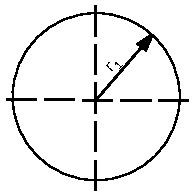
\includegraphics[width=\linewidth]{figures/profile_tube.pdf}
  \end{minipage}%
  \hfill%
  \begin{minipage}{0.8\textwidth}
    \begin{equation}
    \begin{aligned}
      \gamma_{yz} &= \frac{Q_y M_{x}^A*}{b(y) I_x} = \frac{Q}{r^2}\\
      M_{x}^{A_{y=0}} &= \frac{\pi r_1^2}{2} \\
      b(y=0) &= 2 r_1 \\
      I_x &= \frac{\pi r_1^4}{4}
      \end{aligned}
    \end{equation}
  \end{minipage}
  Given a tangent force Q, the shear stress can be calculated.
  If this is over the ultimate strength, the cylinder will break.
  % subsubsection shear_analysis (end)

  \subsubsection{Bending} % (fold)
  \label{ssub:bending}
  The bending analysis follows the one carried out in the section \ref{ssub:profile_study} for a cylinder.
  The equivalent force in this case is given by the tension of the belts, mainly the initial (though there are other tensions that appear when the belts moves for example).
  Due to feasibility reasons and the lack of the appropriate measurements devices, some experimental tests trying different tensions and axes where carried out giving good results with a 3 mm rod or more.
  % subsubsection bending (end)

  \subsubsection{Sizing} % (fold)
  \label{ssub:sizing}
  The studies above have been tested for different diameters of rod starting from the smallest size given by the provider and increasing until both conditions are satisfied, due to the requirements of weight reduction.
  In case of using steel as material, the ultimate strength is supposed to be 250 MPa\footnote{https://en.wikipedia.org/wiki/A36\_steel}.
  And for the case of a rod of 3 mm of diameter, both stresses are under the restrictions.
  Thus, 3 mm rods are going to be used.
  % subsubsection sizing (end)
% section rods (end)
%!TEX root = ../../../../report.tex

\subsection{Finite Element Method (FEM)} % (fold)
\label{sub:finite_element_method}
In the sections \ref{sub:limb_profile} and \ref{sub:rods}, pure mathematical tools have been used to calculate deformations and stresses.
This has been possible due to the simplification of the problem and the simple geometries found.
However, other parts have been analyzed with Finite Element Analysis (FEM), in which the part is subdivided into small volumes and then analyzed individually.
This allows the deformation and stress studies of complex geometries.

As an example, in the figures \ref{fig:fem_foot_iteration_1} and \ref{fig:fem_foot_iteration_2}, the iterative foot design is depicted.
Once the first iteration of the foot was modeled, the design has been changed in order to satisfy a minimum deformation criteria.
However, the designs have always been tested experimentally due to this analysis are under the assumption of isomorphic materials which, in the case of 3D printed parts like the shown in the figures, is not true.
The FEM studies have been used more as a qualitative analysis rather than quantitative.

\begin{figure}[ht]
    \centering
    \begin{subfigure}[b]{0.49\textwidth}
        \includegraphics[width=\textwidth]{figures/fem_5N_1.PNG}
        \caption{FEM analysis in left foot iteration 1}
        \label{fig:fem_foot_iteration_1}
    \end{subfigure}
    \begin{subfigure}[b]{0.49\textwidth}
        \includegraphics[width=\textwidth]{figures/fem_5N_2.PNG}
        \caption{FEM analysis in left foot iteration 2}
        \label{fig:fem_foot_iteration_2}
    \end{subfigure}
\end{figure}

% subsection finite_element_method (end)
%!TEX root = ../../../../report.tex
\subsection{Computer-Aided Design (CAD)} % (fold)
\label{sub:computer_aided_design}

\begin{figure}
    \centering
    \begin{subfigure}[b]{0.49\textwidth}
        \includegraphics[width=\textwidth]{figures/legs_foot.jpg}
        \caption{Left foot}
        \label{fig:left_foot}
    \end{subfigure}
    \begin{subfigure}[b]{0.49\textwidth}
        \includegraphics[width=\textwidth]{figures/legs_hip.jpg}
        \caption{Hip}
        \label{fig:hip}
    \end{subfigure}

    \begin{subfigure}[b]{0.49\textwidth}
        \includegraphics[width=\textwidth]{figures/legs_parts.jpg}
        \caption{Additional designed parts}
        \label{fig:mouse}
    \end{subfigure}
    \begin{subfigure}[b]{0.49\textwidth}
        \includegraphics[width=\textwidth]{figures/legs_pulley.jpg}
        \caption{Left ankle serial spring pulley}
        \label{fig:serial_spring_pulley}
    \end{subfigure}

    \begin{subfigure}[b]{0.49\textwidth}
        \includegraphics[width=\textwidth]{figures/legs_pulley_motor.jpg}
        \caption{Motor pulley}
        \label{fig:motor_pulley}
    \end{subfigure}
    \begin{subfigure}[b]{0.49\textwidth}
        \includegraphics[width=\textwidth]{figures/legs_knee_lower.jpg}
        \caption{Left lower knee}
        \label{fig:lower_knee}
    \end{subfigure}

    \begin{subfigure}[b]{0.49\textwidth}
        \includegraphics[width=\textwidth]{figures/legs_ankle_upper.jpg}
        \caption{Left upper ankle}
        \label{fig:ankle_upper}
    \end{subfigure}
    \begin{subfigure}[b]{0.49\textwidth}
        \includegraphics[width=\textwidth]{figures/legs_hip_lower.jpg}
        \caption{Left lower hip}
        \label{fig:hip_lower}
    \end{subfigure}

    \begin{subfigure}[b]{0.49\textwidth}
        \includegraphics[width=\textwidth]{figures/legs_hip_pinion.jpg}
        \caption{Hip's pinion}
        \label{fig:hip_pinion}
    \end{subfigure}
    \begin{subfigure}[b]{0.49\textwidth}
        \includegraphics[width=\textwidth]{figures/legs_knee_upper.jpg}
        \caption{Left upper knee}
        \label{fig:knee_upper}
    \end{subfigure}
\end{figure}

% subsection computer_aided_design (end)
%!TEX root = ../../../../report.tex
\subsection{Mechanical limits of the joints} % (fold)
\label{sub:mechanical_limits}
The implementation of mechanical limits for the joints obeys to two reasons:
\begin{enumerate}
  \item \textbf{Calibration}: they can be used as starting, known positions for the relative encoders.
  \item \textbf{Security}: a mechanical limit will restrict the movements and prevent any configuration non-natural or dangerous for the physical integrity of the robot.
\end{enumerate}

The Figure \ref{fig:joint_limits_hip} depicts how the mechanical limits of the hip (both left and right) are implemented in the upper part, comprising an angle of 90 + 60 = 150 degrees.
Figure \ref{fig:joint_limits_ankle_upper} shows the upper part of the ankle and how the allowed movement of the foot has a range of 60 + 50 = 110 degrees.
The mechanical limits of the knee are obtained as a combination of the lower and upper components of the joint.
These allow movements of 0 + 120 = 120 degrees as shown in the figures \ref{fig:joint_limits_knee_upper} and \ref{fig:joint_limits_knee_lower}.
The angles of the mechanical limits have been calculated according to the physical limitations in humans.

\begin{figure}[ht!]
    \centering
    \begin{subfigure}[b]{0.49\textwidth}
        \includegraphics[width=\textwidth]{figures/joint_limits_hip.PNG}
        \caption{Joint limits of the hip}
        \label{fig:joint_limits_hip}
    \end{subfigure}
    \begin{subfigure}[b]{0.49\textwidth}
        \includegraphics[width=\textwidth]{figures/joint_limits_ankle_upper.PNG}
        \caption{Joint limits of the ankle}
        \label{fig:joint_limits_ankle_upper}
    \end{subfigure}
\end{figure}    

\begin{figure}[ht!]
    \ContinuedFloat % continue from previous page
    \begin{subfigure}[b]{0.49\textwidth}
        \includegraphics[width=\textwidth]{figures/joint_limits_knee_upper.PNG}
        \caption{Joint limits of the knee: Upper link}
        \label{fig:joint_limits_knee_upper}
    \end{subfigure}
    \begin{subfigure}[b]{0.49\textwidth}
        \includegraphics[width=\textwidth]{figures/joint_limits_knee_lower.PNG}
        \caption{Joint limits of the knee: Lower link}
        \label{fig:joint_limits_knee_lower}
    \end{subfigure}
\end{figure}    

% subsection mechanical_limits (end)

% section mechanics (end)
%!TEX root = ../../../report.tex
\vfill
\section{Software} % (fold)
\label{sec:software}

%!TEX root = ../../../../report.tex

\subsection{Motivation} % (fold)
\label{sub:motivation}
When approaching the task of designing a new robotic platform for the AI department at the Mærsk Mc-Kinney Møller Institute, the current development environment being utilized and its capabilities were studied as a first step.
Nowadays, the simulation and control of the robots at the department is based on the LPZrobots \cite{lpzrobots} and Gorobots \cite{gorobots} packages.
These software tools provide both a simulation engine for robots built on ODE \cite{ode}, OSG \cite{osg} and a framework for an easy implementation of controllers in both simulation and hardware.
However, their specificity compared to other existing instruments collides with some of the core design ideas of the robot framework presented here, which are simplicity of use and generalization.
The above mentioned are the reasons why it was decided to migrate the development environment to ROS Jade \cite{ros} for the bipedal locomotion study framework of RuBy. 

% subsection motivation (end)
%!TEX root = ../../../../report.tex

\subsection{ROS control} % (fold)
\label{sub:ros_control}

% subsection ros_control (end)
%!TEX root = ../../../../report.tex
\subsection{ROS control-locokit hardware interface} % (fold)
\label{sub:ros_control_hardware_locokit_interface}

%initialization of enconders for sensory feedback!

% subsection ros_control_hardware_locokit_interface (end)
%!TEX root = ../../../../report.tex

\subsection{Example controllers} % (fold)
\label{sub:example_controllers}
From the \textit{Controller manager} from ROS Control, different joint controllers can be handled.
In the example controllers the position controller and the effort controllers are used individually for each joint.
This joint controllers offer then a topic (e.g. /rubi/left\_ankle\_position) that the user can use to move the actuators.
This are created from a unique package called \textit{rubi\_joint\_controllers}.
It is worth to say that the position controllers are implemented with a PID and that these values have been adjusted experimentally with the simulations for each joint.

Two type of controllers are given that show a different range of options to use with the robot.
Both are gathered in a sole package called \textit{rubi\_controllers}, which gives a more tidy and resource-shared environment rather than having a package for each controller.
This also makes really easy the deployment a new controller by removing all the creation process of a new package.
In order to start a new piece of code this must be created and then added in the \textit{CMakeLists.txt} from where also some examples are included.

The presented code follows the ROS conventions and the code style is the \textit{Google style} offered by the clang-code-model.
This creates a congruent workspace supervised by a git repository.

\subsubsection{Two neuron controller} % (fold)
\label{ssub:two_neuron_controller}
This first example controller shows how to:
\begin{enumerate}
    \item Use GoRobots.
    \item Make use of dynamic reconfigure.
    \item Adapts its behavior depending on gazebo real time factor.
\end{enumerate}
For the first, an example of how to link C++ code from GoRobots is shown in the \textit{CMakeLists.txt}.
This system is easier and more powerful than the current \textit{Makefiles} currently used in GoRobots.
The Artificial Neuronal Network (ANN) library is used to create a bi-neuronal network that creates the CPG signals of the actuators.
Furthermore, the synaptic weights can be modified by making use of the ROS feature \textit{Dynamic Reconfigurable Parameters}.
These offer an interface in order to change, on the fly, the the values of the created parameters.
In the Figure \ref{fig:rqt_interface}, an RQT workspace containing the CPG signals and the dynamic reconfigurable parameters modifiers is depicted.

\begin{figure}[tb]
    \centering
    \includegraphics[width=\textwidth]{figures/rqt_interface}
    \caption{RQT workspace containing the CPG signals and the dynamic recofigurable parameters.}
    \label{fig:rqt_interface}
\end{figure}

This are also used to change the behavior of the ANN in order to be adapted to changes in Gazebo.
Gazebo uses can accelerate and decelerate the speed at which the time is passing through.
This is adjusted with a \textit{real time factor} that is read by the node and used to adjust the frequencies of the CPGs.
% subsubsection two_neuron_controller (end)

\subsubsection{Impulse controller} % (fold)
\label{ssub:impulse_controller}
Among other things this node shows how to:
\begin{enumerate}
    \item Load and unload different joint controllers.
    \item Give some wrappings for set of controllers (hoping position).
    \item Offer services for jumping: given a file or given the values and impulse time.
\end{enumerate}
This node implements some methods that enable it to change on-the-fly the controllers of each individual joint.
Furthermore, three combinations of individual joint controllers are given being these: (1) all in position mode, (2) all in effort mode and (3) left leg in position mode and right in effort mode.
The last one is useful when hoping, a moment in which a leg must hold a position and the other keep pushing in order to jump.

Three different services are implemented that impulse the robot in the sake of rise it from the floor.
The first two, are \textit{impulse\_one\_leg} and \textit{impulse\_two\_legs} which given a torque for each joint and an impulse time, it gives the possibility to jump either with one or two legs.
Both services load the necessary joint controllers in order to achieve the desired movements.
The third one offers sort of the same service but the parameters are read from a file instead.
This is handy when combined with the dynamic controller developed in MatLab and explained in the section \ref{sec_dynamic_model}.
% subsubsection impulse_controller (end)

% subsection example_controllers (end)

% section software (end)

% chapter design (end)chapters/cha_design/
    %!TEX root = ../../report.tex
\chapter{Simulation} % (fold)
\label{cha:simulation}
Within the goals of the framework is the creation of an ecosystem among software and hardware whose last target is to facilitate the researcher the test of new controllers.
The process of testing new code in locomotion is usually slow due to the inherent problems of the hardware: maintenance, adjustments, bringing up the robot...
Which breaks the workflow of the user and force to spend a time that should be used in the actual development of the program.
The RuBi framework includes a simulator and its simulation model in order to tackle this problem.
The sections of this chapter include from a comparison of simulators to the explanation of how to start developing, passing through the creation of the robot and other tools implemented like dimensional analysis or a rotational holder for the device.

%!TEX root = ../../../report.tex
\section{Motivation} % (fold)
\label{sec:sim_motivation}
What is a simulator, why to simulate

% section motivation (end)
%!TEX root = ../../../report.tex
\section{Comparison of simulators} % (fold)
\label{sec:sim_comparison_of_simulators}
When choosing a simulation platform there are several factors to have into account.
Three robotic simulators have been analyzed and compared. 
These are: LPZ Robots \cite{lpzrobots} (Figure \ref{fig:lpzrobots_example}), V-Rep \cite{vrep} (Figure \ref{fig:vrep_example}) and Gazebo \cite{gazebo} (Figure \ref{fig:gazebo_example}).
Some comparisons can be found in the literature as \cite{nogueiracomparative} or \cite{staranowicz2011survey} however the predominant criteria has been their integration with ROS.

\begin{figure}[hb!]
  \begin{subfigure}{.33\textwidth}
    \centering
    \includegraphics[width=.95\linewidth]{figures/vrep_example}
    \caption{V-Rep example}
    \label{fig:vrep_example}
  \end{subfigure}%
  \begin{subfigure}{.33\textwidth}
    \centering
    \includegraphics[width=.95\linewidth]{figures/lpzrobots_example}
    \caption{LPZ Robots example}
    \label{fig:lpzrobots_example}
  \end{subfigure}
  \begin{subfigure}{.33\textwidth}
    \centering
    \includegraphics[width=.95\linewidth]{figures/gazebo_example}
    \caption{Gazebo}
    \label{fig:gazebo_example}
  \end{subfigure}
  \caption{Simulation examples of the software analyzed}
  \label{fig:simulation_comparison}
\end{figure}

The RuBi robot is mainly targeted to be used in the AI department at the Maersk Mc-Kinney Møller Institute, where the toolbox GoRobots is being developed.
This is a set of tools, from a neuronal networks API to a genetic algorithm engine, written in C++ than is meant to be simulator-independent.
However, in order to provide a more general and supported simulation and development environment for the user, ROS Jade \cite{ros} has been selected as the tool to use.
The whole set of instruments provided in ROS along with its easy extendability give the opportunity to use the controllers and tools already developed in GoRobots.
Despite the fact that the three simulators compared have a C++ interface that would allow to interface them with ROS, Gazebo is already fully supported and integrated in ROS, making it the logic choice.
This reduces the learning curve of a new user and the installation process is easier due to it is included in the Open Source Robotics Foundation (OSRF) repositories.

Regarding the second condition, Gazebo has the feature of changing the physics engine in the beginning of the simulation, it has multiphysics support (fluids, electromagnetism...), it allows to load external geometries from STL or Collada and, the most important, has an active community behind it providing support and documentation. These are the reasons for selecting Gazebo as the simulator for the RuBi platform.
In \cite{physics_engine_gazebo_comparison}, a comparison with the different physical engines is carried out.
For the sake of simplicity the default one, Open Dynamics Engine (ODE), has been used, although the others have been tested.

% section comparison_of_simulators (end)\[
%!TEX root = ../../../report.tex
\section{Robot definition} % (fold)
\label{sec:robot_definition}
SDF vs URDF vs Xacro

% section robot_definition (end)
%!TEX root = ../../../report.tex
\section{Robot model creation} % (fold)
\label{sec:robot_creation}
One of the goals of the framework is to facilitate its further use and development.
For this reason this section is dedicated to explain how the robot model was created for Gazebo, so that it can be modified in the future.

A robot is defined as a set of links joined, where a link contains at least three blocks of information:
\begin{enumerate}
   \item The collision model: used to calculate the collisions with other agents in the simulation.
   \item The visual model: uniquely used for visual purposes.
   \item The inertial information: defines physical properties like the mass and the moments of inertia of the link.
\end{enumerate} 

A trade-off must be found for the precision of the collision model between accuracy and speed.
The more detailed is the model, the more accurate its simulation will become, but this implies a higher computational load and processing time.
The general advice is to have two simulation models: one for visual purposes and the other one for collisions.
In the case of the frame of RuBi the visual models are obtained directly by exporting the parts from SolidWorks, while the collision models are made out of primitive gazebo shapes (cubes, cylinders, spheres...) for the whole body except the feet.
Since the robot is not meant to collide with obstacles due to its nature and setup, the possible collisions in the body are not a priority, then each link is represented as a cylinder of the same length of the CAD model and of a radius enough to cover the whole part.
An example can be seen in the Figure \ref{fig:collision_model}.

The moments of inertia of each individual link are obtained directly from SolidWorks.
The CAD model includes the materials and thus the masses.
From these, the program is able to calculate the moments of inertia.
The Figure \ref{fig:moments_of_inertia} shows the representation of these parameters in the simulation.


\begin{figure}[hb!]
  \centering
  \begin{subfigure}{.45\textwidth}
    \centering
    \includegraphics[width=.5\linewidth]{figures/gazebo_collision_model.png}
    \caption{Gazebo showing the visual model, the moments of inertia and the collision model.}
    \label{fig:collision_model}
  \end{subfigure}
  \begin{subfigure}{.45\textwidth}
    \centering
    \includegraphics[width=.5\linewidth]{figures/gazebo_intertia_moments.png}
    \caption{Gazebo showing the visual model and the moments of inertia.}
    \label{fig:moments_of_inertia}
  \end{subfigure}
  \caption{Gazebo showing physical and visual propperties of RuBi.}
\end{figure}

It is essential to make sure that the visual models and moments of inertia are exported referred to the correct coordinate systems.
In the case of the ankle, for example, the STL file and the moments of inertia are calculated from the coordinate system whose origin is positioned in the middle of the rotational axis of the joint, with its Z axis attached to the rotational axis and Y pointing to the biggest extension of the part.
This can be seen in the Figure \ref{fig:solidworks_ankle_coodinate_system}.

\begin{figure}[ht!]
  \centering
  \includegraphics[width=0.75\linewidth]{figures/solidworks_ankle_coordinate_system}
  \caption{Coordinate system of the left ankle in SolidWorks.}
  \label{fig:solidworks_ankle_coodinate_system}
\end{figure}

Finally, in the Xacro file the information that lacks the URDF must be added in order to simulate with Gazebo.
To do so, the following has to be added to the RuBi description:
\begin{enumerate}
  \item \textbf{Plug-in for ROS Control}: Offers an interface for using ROS Control inside Gazebo.
  \item \textbf{Contact sensors}: Simulates contact sensors as in the feet of the real robot.
  \item \textbf{Friction coefficients}: Defines the friction between the feet and the floor.
\end{enumerate}

The robot has been simulated with direct drive transmission, since the springs configurations has not been implemented because of the lack of time.
This is left as further work.

% section robot_creation (end)
%!TEX root = ../../../report.tex
\section{Dimensional analysis} % (fold)
\label{sec:dimensional_analysis}
A problem came up when creating the robot. 
Some of the inertia moments obtained from SolidWorks, were in the order of magnitude of $10^{-8}$.
Such small number is not handled by the physics engine correctly causing the robot model to be unstable under normal conditions.

Three approaches were taken:
\begin{enumerate}
  \item \textbf{Change the physics engine}: As commented in the simulation comparison \ref{fig:simulation_comparison}, Gazebo supports multiple physics engines. Dart \cite{dart}, Simbody \cite{simbody}, Bullet \cite{bullet} and ODE \cite{ode}, where tested giving the same unstable behavior. 
  Thus, this method was discarded.
  \item \textbf{Fake the moments of inertia}: This would be to make 0 the really small moments of inertia and only leave the ones over a threshold.
  As the simulation is a qualitative analysis and no quantitative, an exact match of the moments of inertia is not needed. 
  \item \textbf{Dimensional analysis}: Based on \cite{dimensional_analysis}, the size of the robot can be increased in a proportion that make the figures big enough to be handled.
\end{enumerate}

Dimensional analysis can be applied to correlate the physical properties of the original robot with its scaled replica.
This is, if the original robot with mass $m$, volume $V$ and moment of inertia about an axis $I$, given a scale factor $s$, calculate the scaled replica $m'$, $V'$, $I'$ depending exclusively on $s$.

In the equation \ref{eq:general_inertia}, the generalized expression of the moment of inertia about an axis is shown.
\begin{equation}
\label{eq:general_inertia}
  I = \iiint_V \rho(u,v,w) |r^{2}| \,dx\,dy\,dz
\end{equation}

If the equation \ref{eq:general_inertia} is taken as the moment of inertia from the first link, the scaled one would be the shown in the equation \ref{eq:general_inertia_2}:
\begin{equation}
\label{eq:general_inertia_2}
  I' = \iiint_{V'} \rho(u,v,w)' |r^{'2}| \,dx'\,dy'\,dz'
\end{equation}

Supposing a scale factor of $s$ and as stated in the equations from \ref{eq:dx} to \ref{eq:dz}:

\begin{multicols}{3}
  \begin{equation}
  \label{eq:dx}
    \,dx=s \,dx'
  \end{equation}\break
  \begin{equation}
  \label{eq:dy}
    \,dy=s \,dy'
  \end{equation}\break
  \begin{equation}
  \label{eq:dz}
    \,dz=s \,dz'
  \end{equation}\break
\end{multicols}

Then can be deduced that $r$ increases proportionally with $s$ as shown in the figure \ref{fig:dimensional_analysis} and presented in the equation \ref{eq:dr}:
\begin{equation}
  \label{eq:dr}
  \,r=s \,r'
\end{equation}

\begin{figure}[ht!]
  \centering
  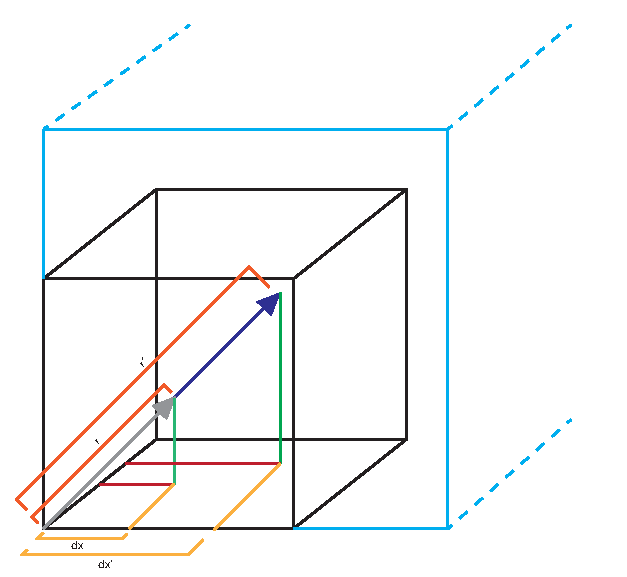
\includegraphics[width=0.5\linewidth]{figures/dimensional_analysis.pdf}
  \caption{Representation of a minimal volumentric cube.}
  \label{fig:dimensional_analysis}
\end{figure}

Assuming a constant density across all the scaled bodies, and particularizing for the moment of inertia of the center of gravity the moment of inertia is given then by \ref{eq:general_inertia_3}:
\begin{equation}
  \label{eq:general_inertia_3}
  I'_{CG} = \iiint_{V'} \rho(u,v,w)' |r^{'2}| \,dx'\,dy'\,dz' = s^{3} r_{CG}^{'2} m
\end{equation}

A correlation can be obtained for the inertia then as shown in \ref{eq:inertia_scale}:

\begin{equation}
\label{eq:inertia_scale}
  I' = \frac{s^{3} r_{CG}^{'2} m}{r_{CG}^{2} m} I = s^{5} I
\end{equation}

And lately the mass can be correlated as in \ref{eq:mass_scale}:
\begin{equation}
\label{eq:mass_scale}
  m' = V' \frac{m}{V} = s^{3}m
\end{equation}

As explained in the \ref{sec:robot_definition}, by using the Xacro format, mathematical expressions can be used.
The definition of the robot includes a set of variables in which is included $scale$ that is used to calculate $mass\_scaled$ and $inertia\_scaled$ that will modify the values of all the links to make a coherence scalable robot definition.

% section dimensional_analysis (end)
%!TEX root = ../../../report.tex
\section{Environment creation} % (fold)
\label{sec:environment_creation}
Talk about the rotational robot holder, the trade mill, other possible environment.

% section environment_creation (end)
%!TEX root = ../../../report.tex
\section{How to simulate} % (fold)
\label{sec:how_to_simulate}
The actions for starting the simulation are minimal and, with everything installed, just a terminal shall be opened and the user have to insert:

\begin{lstlisting}
roslaunch rubi_gazebo rubi_world.launch
\end{lstlisting}

The launch file will load ROS Control along with the simulation.
From that moment the user can run the controllers and the legs will move equally than in the real robot.
% section how_to_simulate (end)
% chapter simulation (end)

    %!TEX root = ../../report.tex
\chapter{Construction process} % (fold)
\label{cha:implementation}
This chapter is dedicated to explain the process of manufacturing and assembling the introduced designs.
From the important role of emerging low-cost technologies like FFF 3D printing up to the creation of custom PCBs for reducing the weight of the robot, the following sections are meant to explain the process of acquisition and construction of all the components of RuBi presented in previous chapters.
The implementation of the final prototype has always been led by criteria of security, constrained budget and feasibility for maintenance and futures improvements.

%!TEX root = ../../../report.tex
\section{3D printing} % (fold)
\label{sec:3d_printing}
The parts modeled for the project and shown in section \ref{sub:computer_aided_design}, have been printed using Fused Filament Fabrication (FFF).
The 3D printer used is a M Prime One \footnote{https://github.com/M-Prime/M\_Prime\_One} with a 0.4 mm noozle.
All the parts have been printed at 0.2 mm layer height.

The use of this technology is justify by the fact that makes the iterative process between design and manufacturing both fast and cheap. \todo{Fast and low-cost prototyping}
All the parts have been individually adjusted until the clearances have been as expected.
Furthermore, this enable the user not only to replicate the parts with out any considered extra cost, but allows the robot to be easily replicated in other places.

When manufacturing, some of the parts have needed material support.
\todo{Why the material support? Tell how you've managed to print the most complex stuff}
The figure \ref{fig:photo_material_support} depicts two feet, one with material support and the other with it removed.
In the figure \ref{fig:photo_3d_printed} a detail of actual parts 3D printed and assembled in the robot are shown.

\begin{figure}[ht]
    \centering
    \begin{subfigure}[b]{0.49\textwidth}
        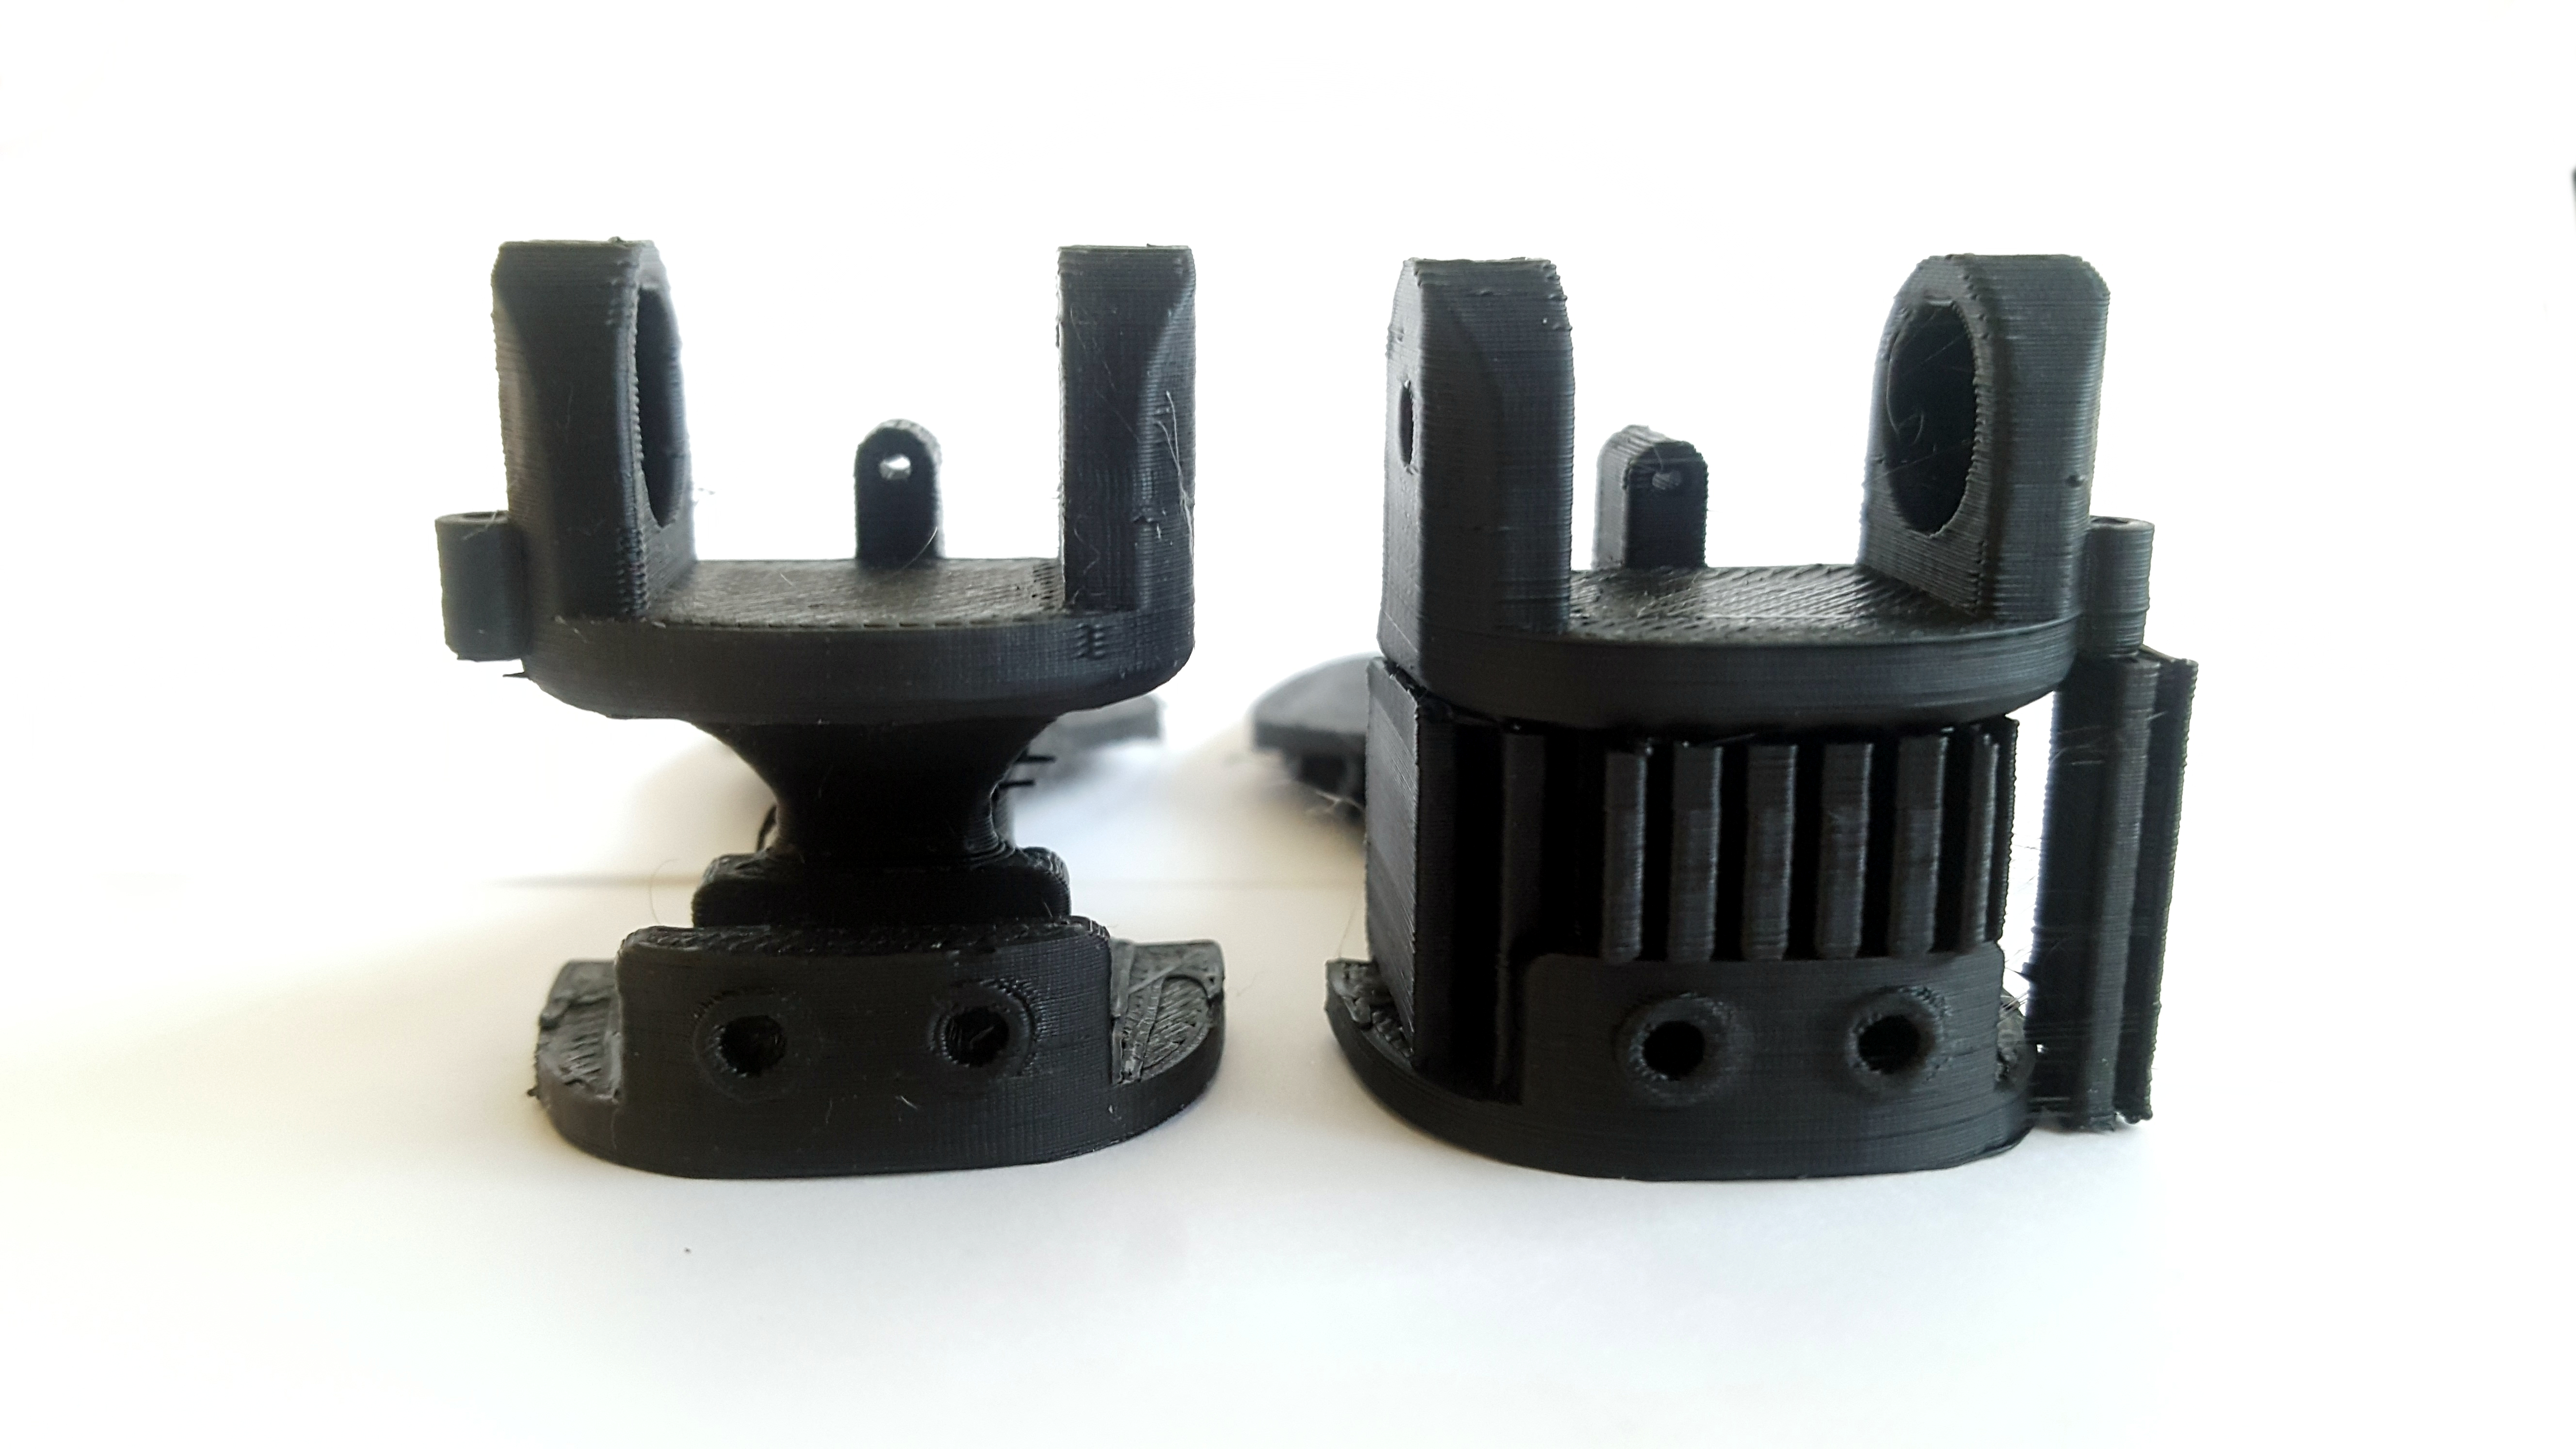
\includegraphics[width=\textwidth]{figures/photo_material_support.jpg}
        \caption{Feet with and without material support}
        \label{fig:photo_material_support}
    \end{subfigure}
    \begin{subfigure}[b]{0.49\textwidth}
        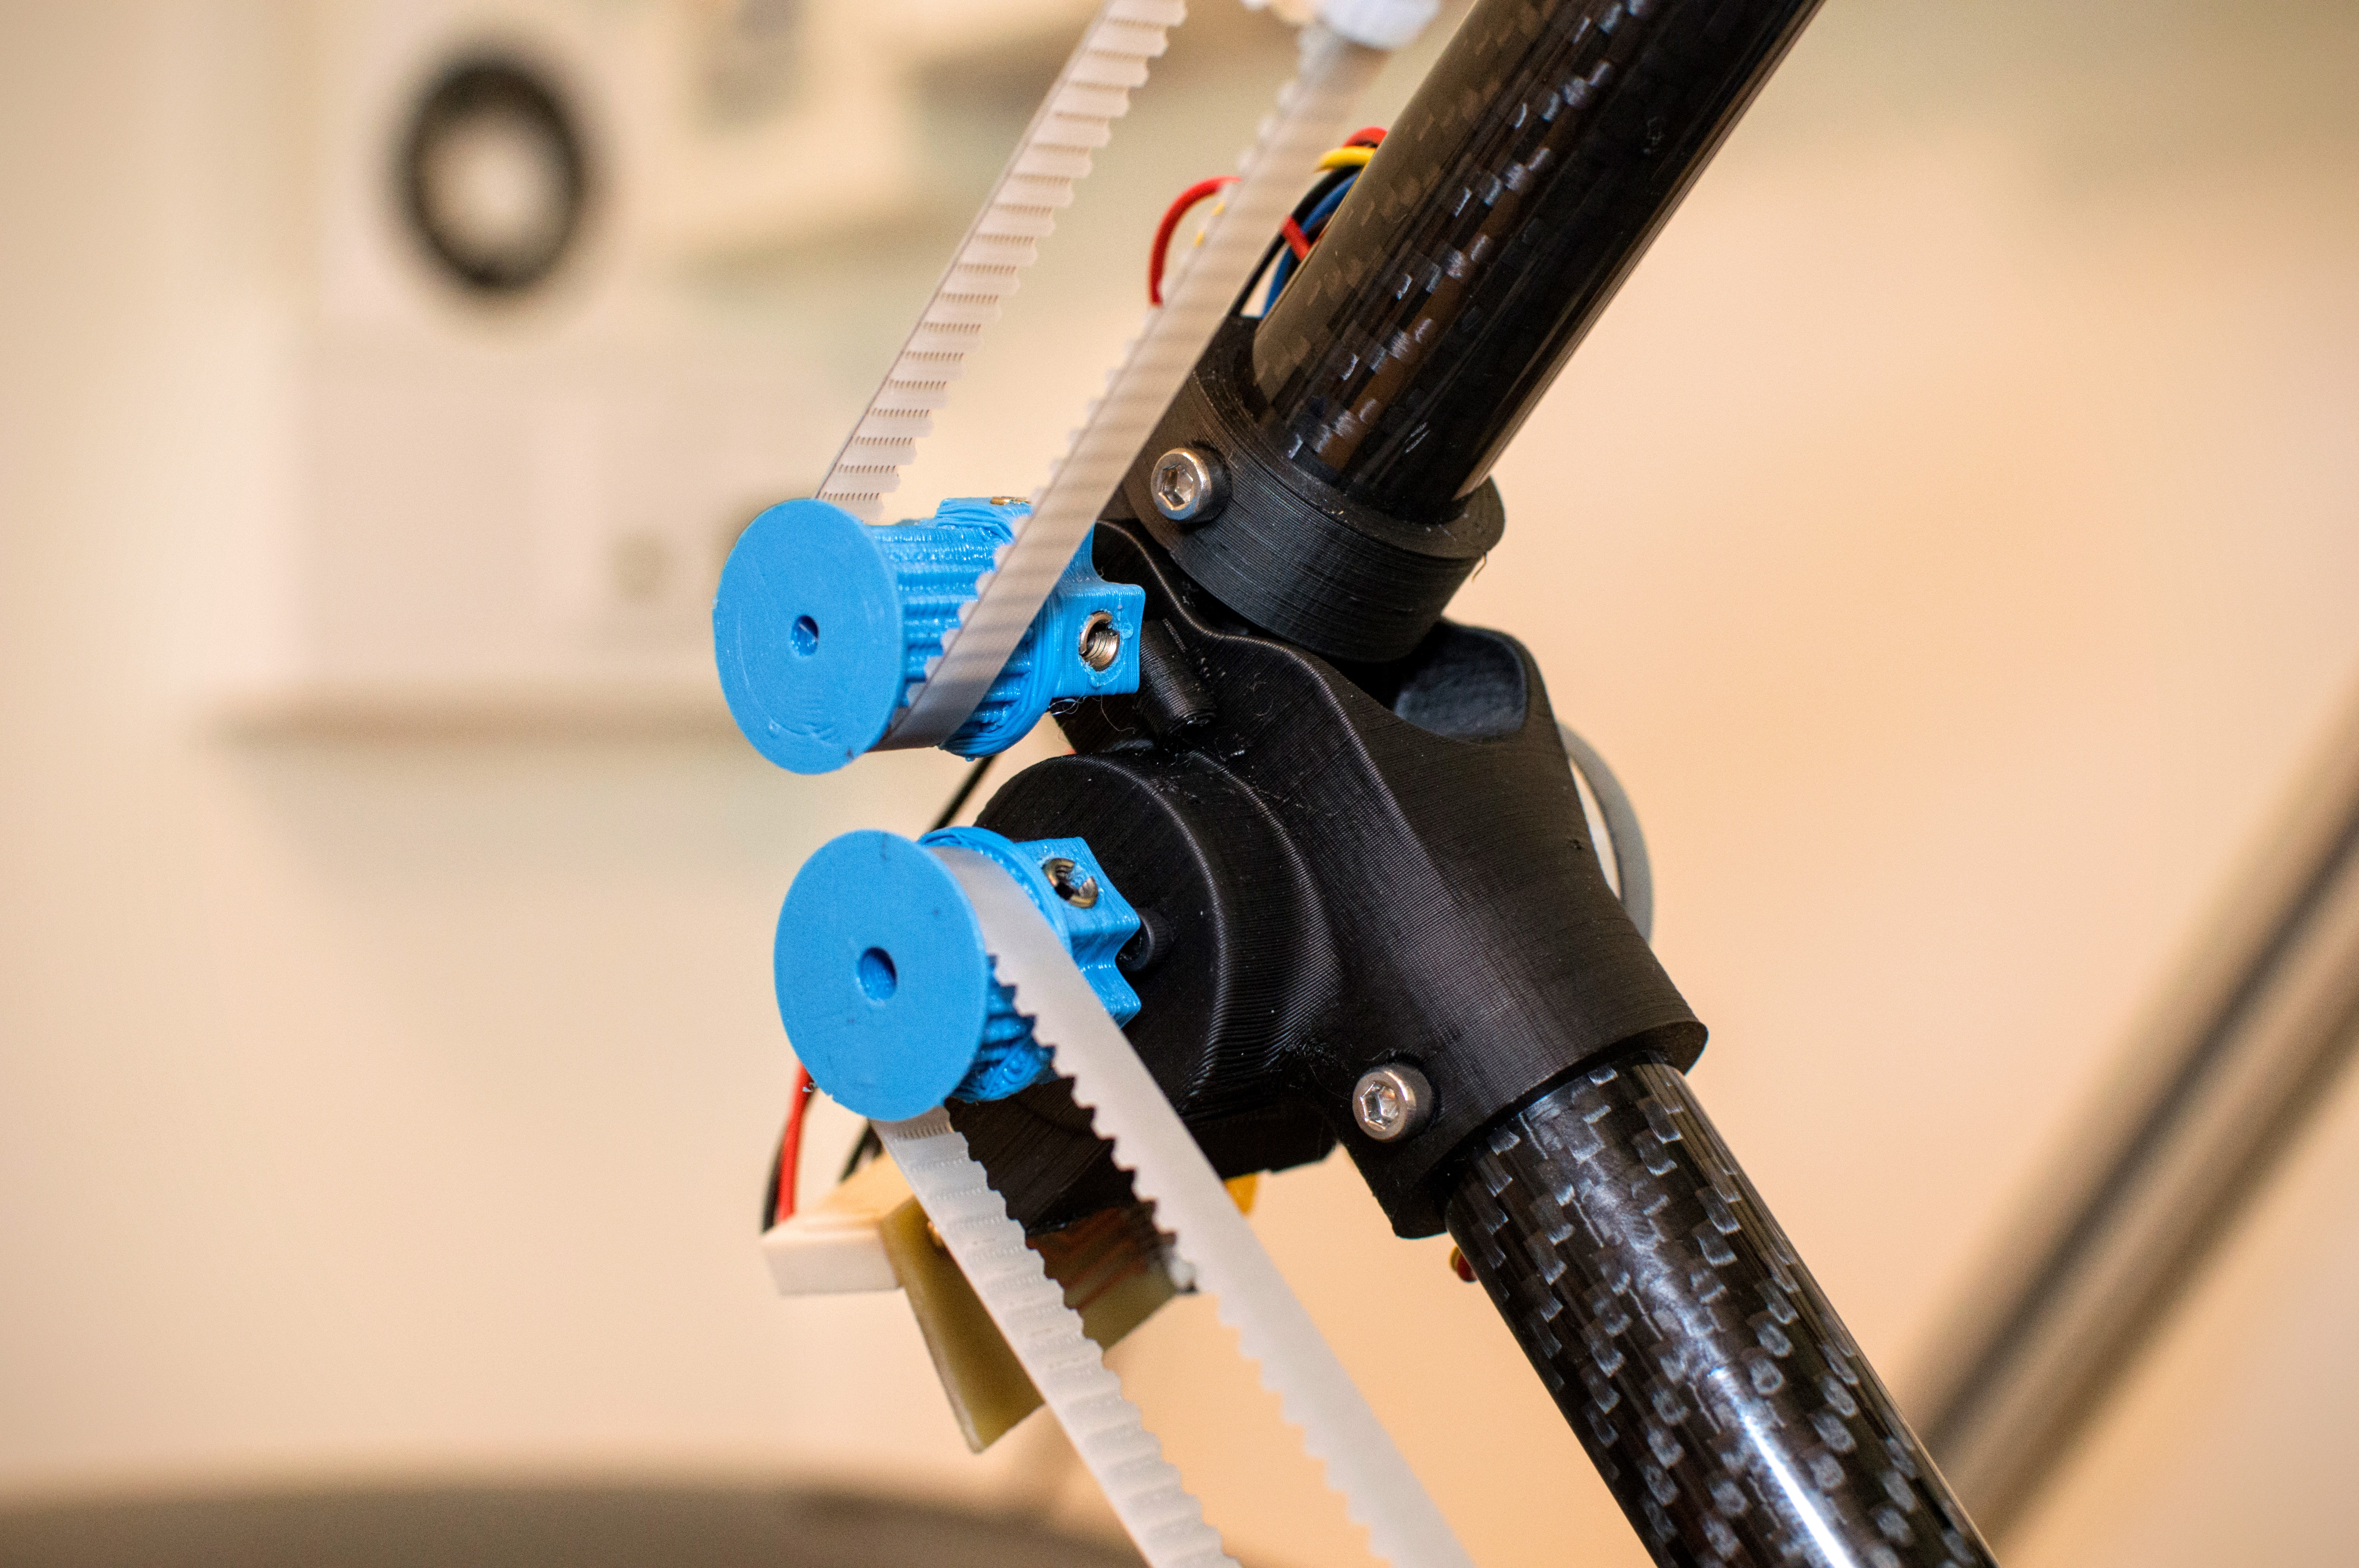
\includegraphics[width=\textwidth]{figures/photo_3d_printed.jpg}
        \caption{Detail of 3D printed parts assembled}
        \label{fig:photo_3d_printed}
    \end{subfigure}
\end{figure}

  \subsection{Arc compensation} % (fold)
  \label{sub:arc_compensation}
  For the CAD models of the 3D printed parts, the clearances of the internal holes have been adjusted following \cite{arc_compensation}.
  The undersizing of internal holes is a common problem in this sort of technology due to the lack of information of the common-used exporting format: the STL.
  This only contains the 3D model expressed as a set of external triangles, which difficult the correction of malformations inherent to the technology.

  In the case of the Fused Filament Fabrication (FFF), the material is extruded equally in both sides of the arc, as shown in \ref{fig:arc_compensation}. 
  However, in the side of the smaller curve, less material is needed.
  This correction can be calculated with:

  \todo{Label and reference the equations}
  $$ r=\frac{t+\sqrt{t^2+4R^2}}{2}$$

  being:
  \begin{enumerate}
    \item t: noozle diameter
    \item R: desired internal hole radius
    \item r: corrected radius
  \end{enumerate}
  As an example, Klee suggests an internal hole of 4.4 mm in the case of the selected nuts \cite{klee}. Thus, the diameter in the CAD model has been adjusted for this data and a noozle of 0.4 mm. The result is then:
  $$ d=2r=\frac{t+\sqrt{t^2+4R^2}}{2}=0.4+\sqrt{0.4^2+4*2.2^2}=4.81$$

  \begin{figure}[tb]
    \centering
    \includegraphics[width=0.5\textwidth]{figures/Arc-compensation}
    \caption{Technical representation of the generated arc when using FFF technology}
    \label{fig:arc_compensation}
  \end{figure}
  % subsection arc_compensation (end)

% section 3d_printing (end)
%!TEX root = ../../../report.tex
\section{Machining} % (fold)
\label{sec:machining}
Along with 3D printing, other parts have needed to be machined.
Though its allows the creating of complex geometries, the 3D printers used have a limited printing volume.
Additionally, the mechanical properties given by the PLA do not satisfy all the needs of the used parts.
The rods of the axis, the beams used to create the structure, the carbon fiber tubes are some examples of this requirements of size and mechanical stress.
Special attention has been paid to the symmetry during the construction following the design criteria established in \ref{sec:physical_properties}.

This materials usually come in a raw format that must be then modified in order to get the desired component.
As an example, the rods came in bars of one meter that have been cut and filed according the design.
Other example are the carbon fiber tubes.
These have been designed to carry the wiring inside them.
Thus some holes have been performed in the bottom and top part of the tube in order to insert them.
Knowing that this kind of operations is human error prone, non-critical parts have been machined or no such it can affect to the correct behavior of the device.
Furthermore, the actuation has always tried to be as much correct as possible and always following the appropriate security rules.
The drawings for such parts are included as appendices in \ref{app:mechanical_drawings}.

% section machining (end)
%!TEX root = ../../../report.tex
\section{PCBs and wiring} % (fold)
\label{sec:pcbs_and_wiring}

% section pcbs_and_wiring (end)
%!TEX root = ../../../report.tex
\section{Providers} % (fold)
\label{sec:providers}
In addition to the 3D printed and machined parts, other items have been bought from providers.
The providers have been selected based on previous shoppings made by the Mærsk Mc-Kinney Møller Institute.
All the needed items that could have followed an standard have been chosen. 
As an example, the robot only needs three types of screws and one kind of bearings.
The components are easily found and are not rare items that increase the price of the robot.
A list with all the components bought and its providers is attached as an appendix in \ref{app:order_list}.
% section providers (end)
%!TEX root = ../../../report.tex
\section{Assembly} % (fold)
\label{sec:assembly}
Due to basically all the parts have been somehow connected with a 3D printed parts, and all the tolerances of these have been adjusted individually, the assemble process has been found easy and fast.
The mounting processes has shown to be rapid enough to change some of the parts, as the springs, within minutes.
Furthermore, if any part breaks its creation and replacement is easy enough to reduce the maintenance time and be considered it as one of the main points of the whole platform.
The tension of the belts have been adjusted experimentally as explained in the section \ref{sub:pulleys_and_belts} using the zip ties installed.
In the figure \ref{fig:photo_robot_walking}, the complete robot assembled is shown while in the figure \ref{fig:photo_dacbot}, a size comparison between the Dacbot \cite{dacbot1} and RuBi can be done.

\begin{figure}[ht!]
    \centering
    \begin{subfigure}[b]{0.49\textwidth}
        \includegraphics[width=\textwidth]{figures/photo_robot_walking.jpg}
        \caption{RuBi assembled}
        \label{fig:photo_robot_walking}
    \end{subfigure}
    \begin{subfigure}[b]{0.49\textwidth}
        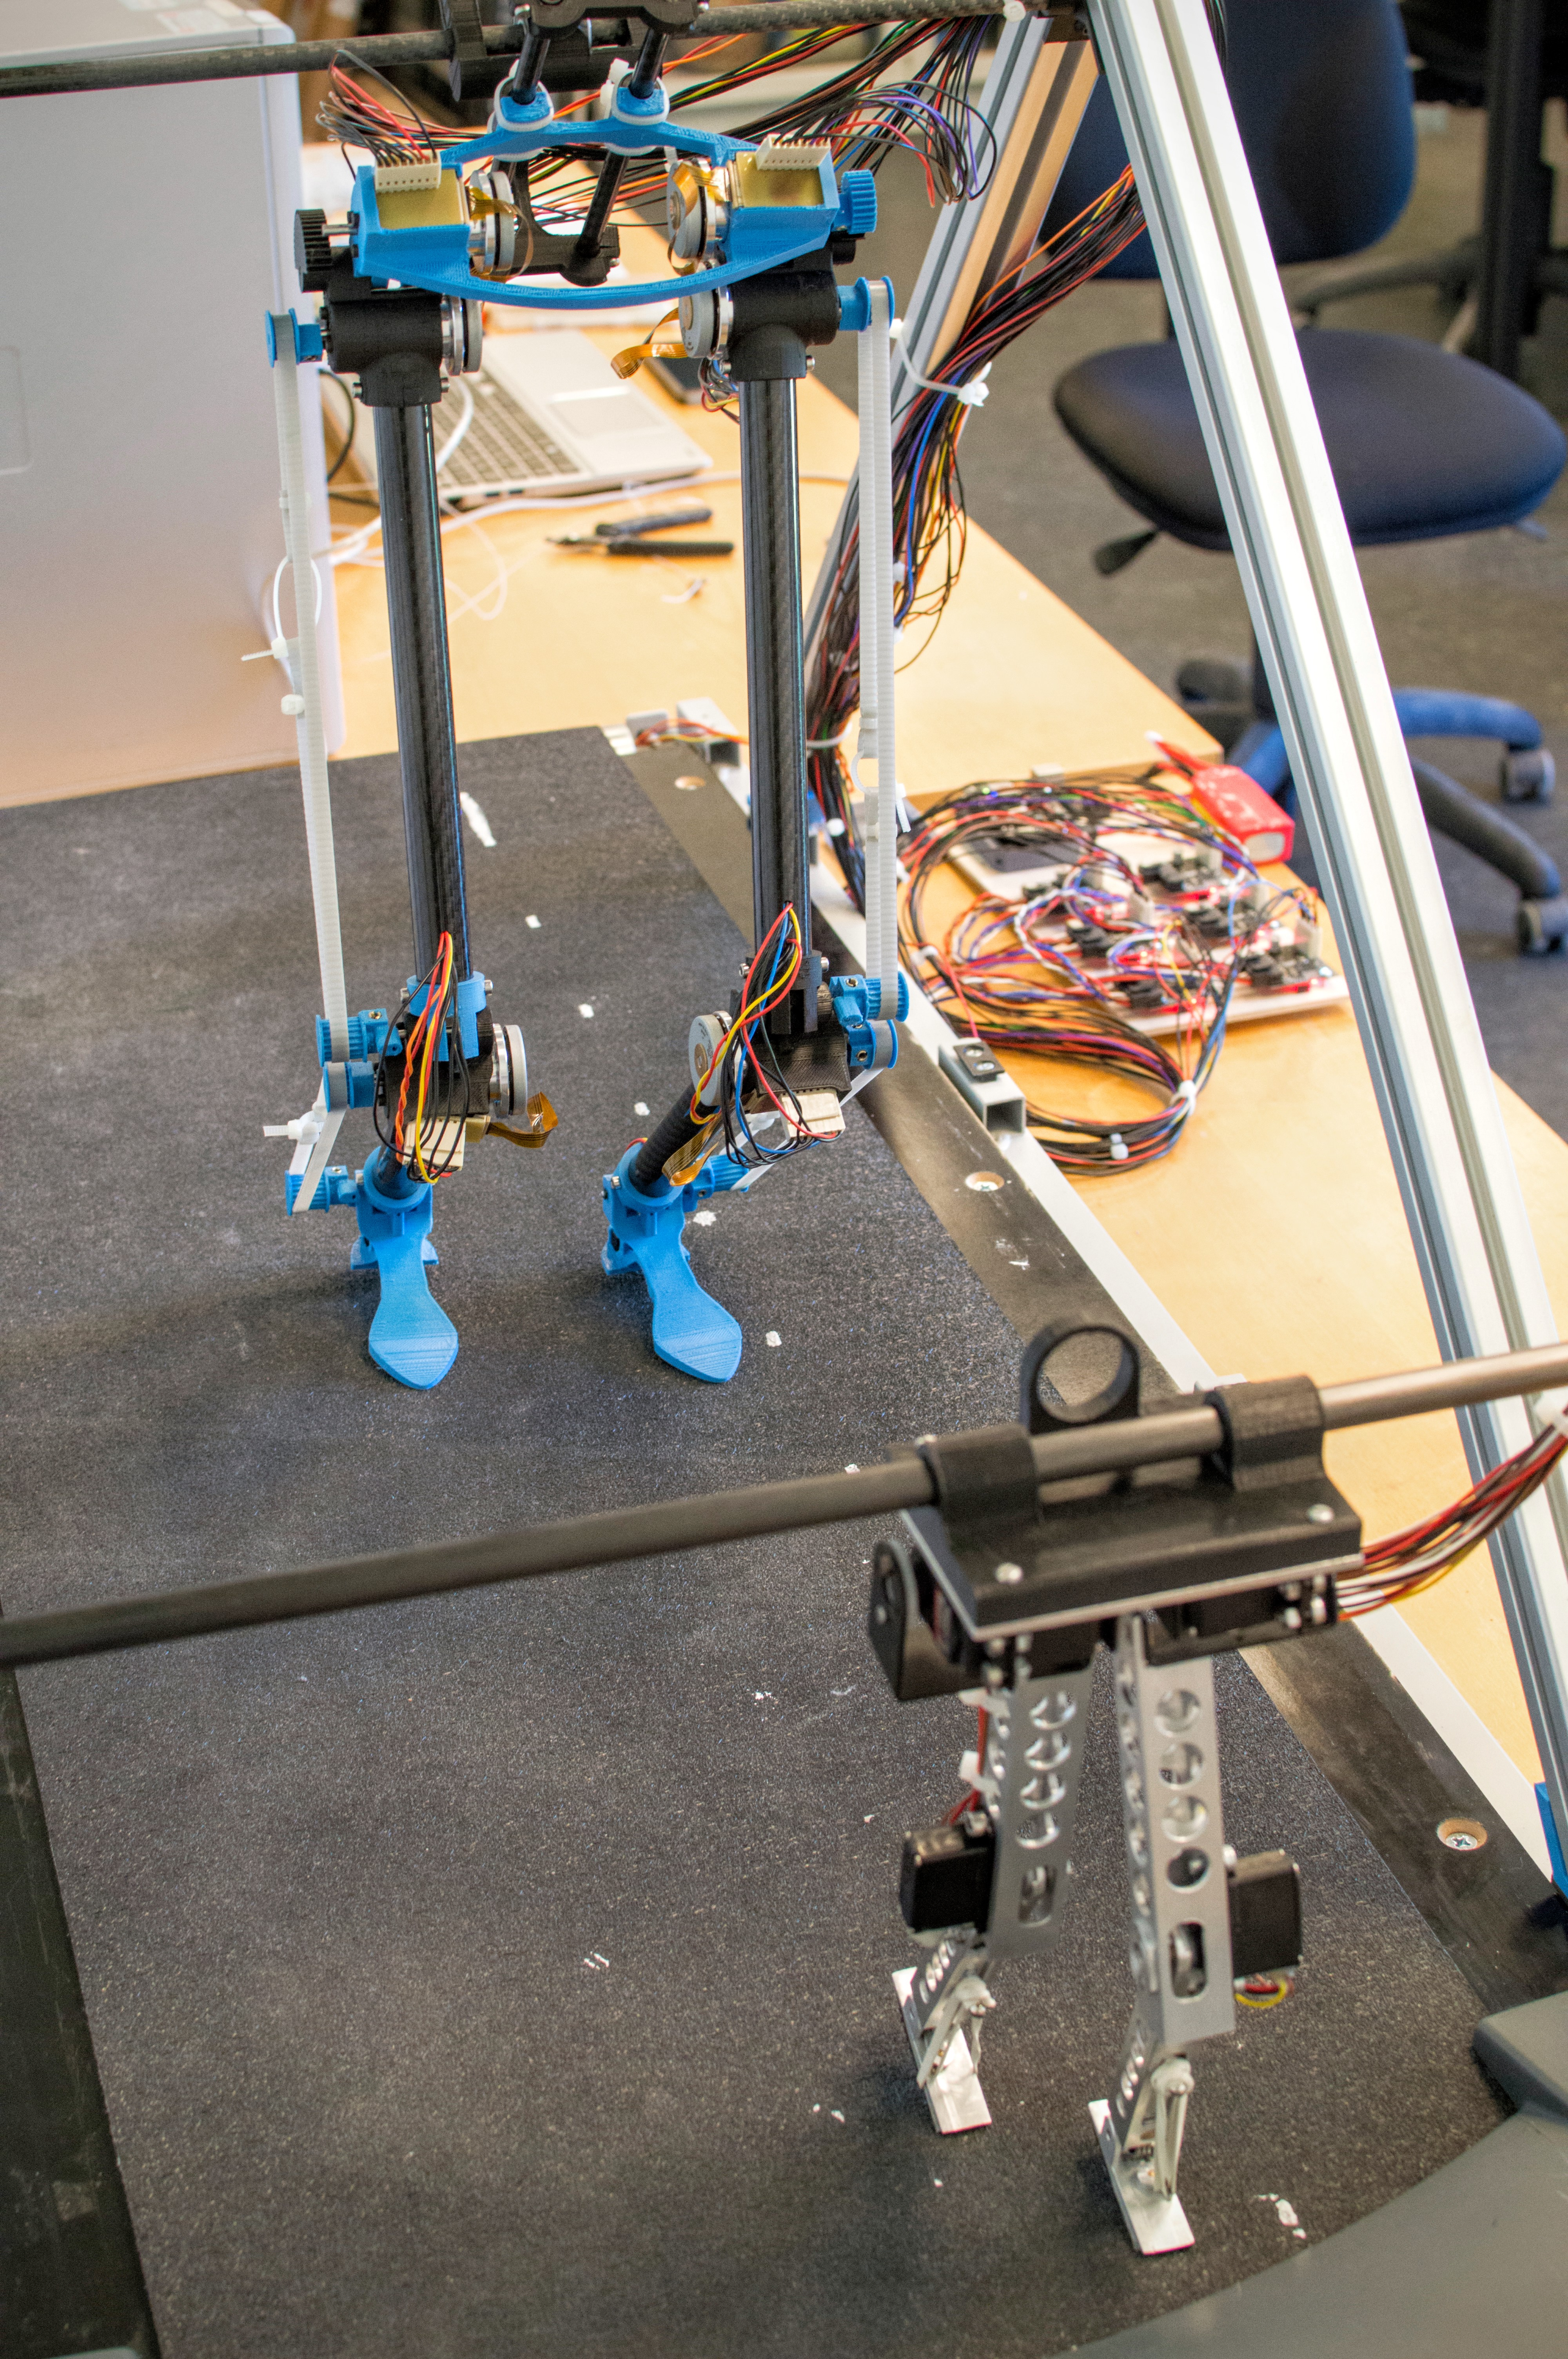
\includegraphics[width=\textwidth]{figures/photo_dacbot.jpg}
        \caption{RuBi and Dacbot over the same treadmill}
        \label{fig:photo_dacbot}
    \end{subfigure}
\end{figure}    
% section assembly (end)
%%!TEX root = ../../../report.tex
\section{How to bring up the robot} % (fold)
\label{sec:how_to_bring_up_the_robot}
In order to bring up the robot, a battery has to power it and the computer must be started.
It will automatically create a Wi-Fi hotspot called \textit{RuBi} where the user can connect to.
From this moment, the robot should be able to receive motor commands.
If not, the IP in the \textit{locokit\_hw} has to be changed according to the stablished in the host.
In the guest, open a new terminal and run:

\begin{lstlisting}
roslaunch rubi_bringup rubi_bringup.launch
\end{lstlisting}

ROS Control will be loaded along with the locokit hardware interface and the controllers can move the real robot.
% section how_to_bring_up_the_robot (end)

% chapter implementation (end)
    %!TEX root = ../../report.tex
\chapter{Experiments} % (fold)
\label{cha:experiments}

\begin{figure}[ht!]
    \centering
    \begin{subfigure}[b]{0.49\textwidth}
        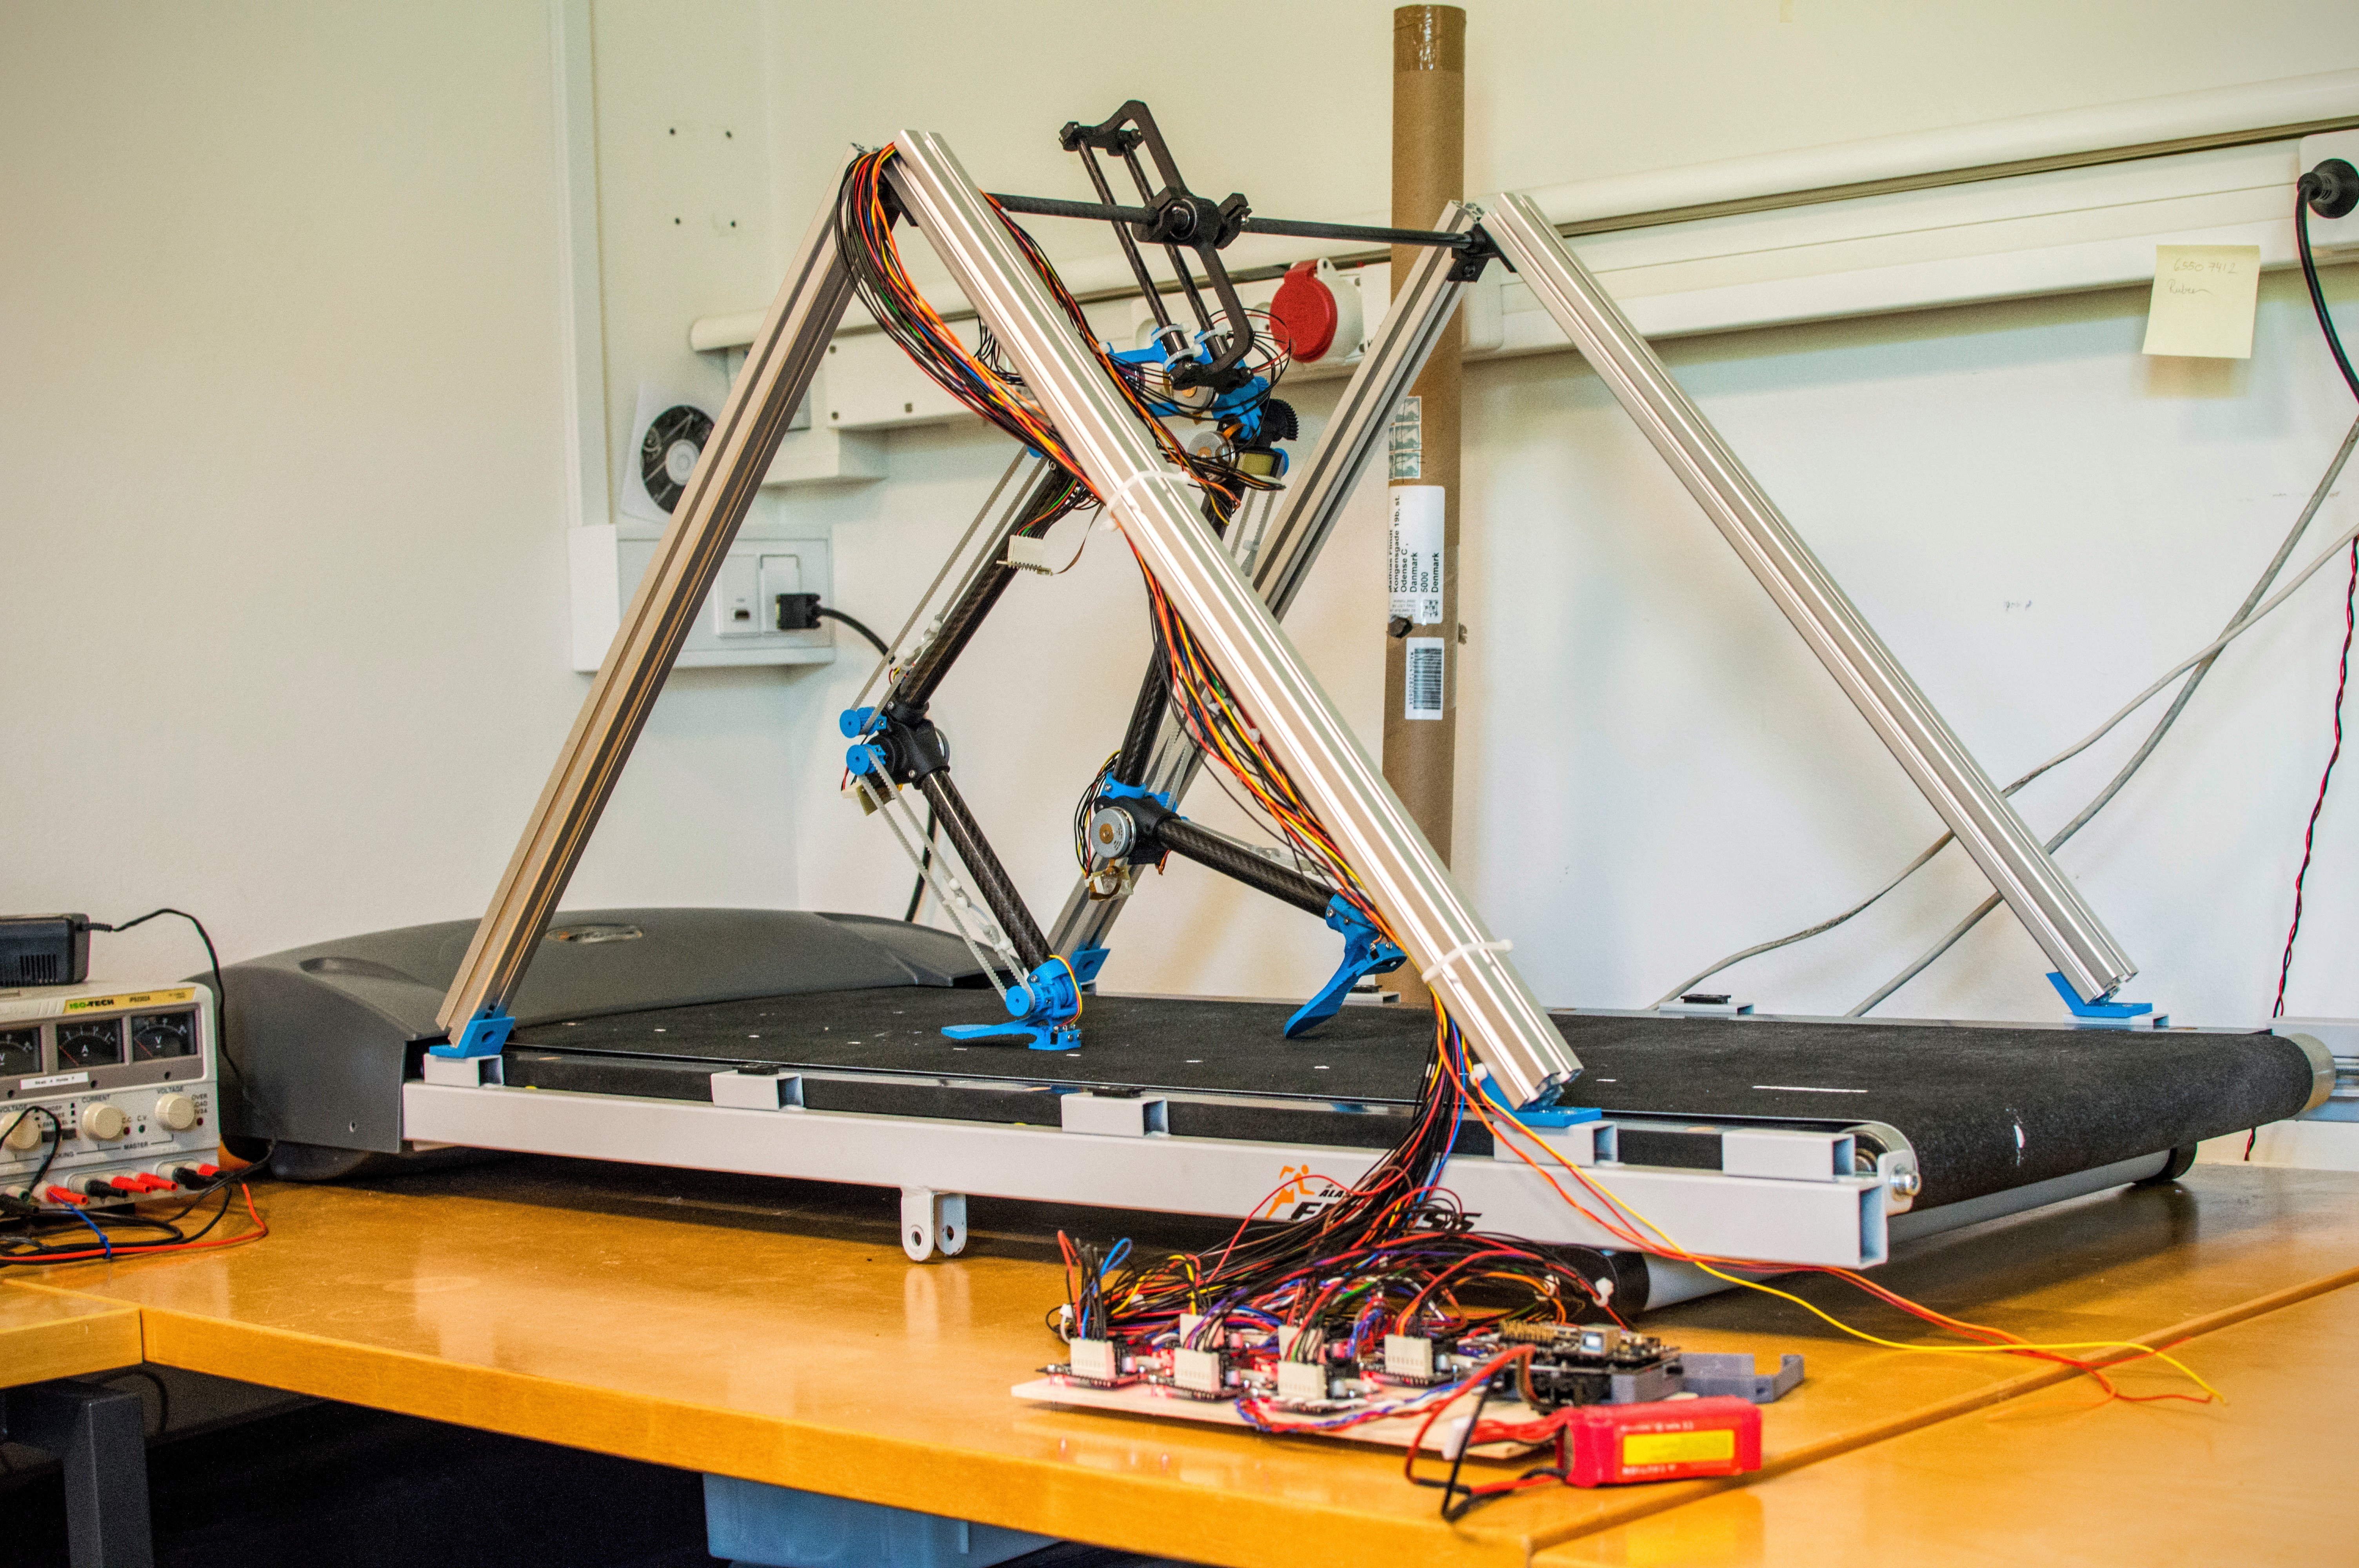
\includegraphics[width=\textwidth]{figures/photo_structure.jpg}
        \caption{RuBi in the test bench assembled}
        \label{fig:photo_structure}
    \end{subfigure}
    \begin{subfigure}[b]{0.49\textwidth}
        \includegraphics[width=\textwidth]{figures/legs_structure.jpg}}
        \caption{Test bench for RuBi rendering}
        \label{fig:legs_structure}
    \end{subfigure}
\end{figure}  

Test bench

% chapter experiments (end)
    %!TEX root = ../../report.tex
\chapter{Economical analysis} % (fold)
\label{cha:economical_aspects}
In this sections the economical aspects of the thesis are detailed.
These are: \textbf{Labor cost} (table \ref{tab:labor_cost}), \textbf{Equipment cost} (table \ref{tab:equipment_cost}), \textbf{Software cost}: (table \ref{tab:sofware_cost}) and \textbf{Material cost} (table \ref{tab:material_cost}).
The depreciation has been calculated using the formula \ref{eq:depreciation}:
\begin{equation}
  \label{eq:depreciation}
  Attriburable\ cost  = \frac{Cost \cdot \% of use \cdot Duration}{Depreciation}
\end{equation}
Some of the values found in the next tables are induced from other data or extracted from forums which make this results, not as quantitative data, but qualitative.
The table \ref{tab:material_cost}, is further detailed in the appendix \ref{app:order_list}, however it include some items that were not ordered (e.g. a Locokit Kit or a 3D printer PLA spool).

\begin{table}[htbp]
\caption{Labor cost}
\centering
\begin{tabular}{l|l|r|r|r}
\multicolumn{ 5}{c}{\Large Labor Cost} \\
\multicolumn{1}{c|}{\textbf{Full Name}} & \multicolumn{1}{c|}{\textbf{Category}} & \multicolumn{1}{c|}{\textbf{\parbox{2.5cm}{ \centering Dedicated hours [h]}}} & \multicolumn{1}{c|}{\textbf{\parbox{2.5cm}{ \centering Cost per hour [DKK/h]}}} & \multicolumn{1}{c}{\textbf{Cost [DKK]}} \\ \hline
Jorge Rodriguez & Engineer & 120 & 130 & 15600 \\ \hline
Ignacio Torroba & Engineer & 120 & 130 & 15600 \\ \hline
Jørgen Christiensen & Senior Engineer & 20 & 200 & 4000 \\ \hline
Poramate  & Senior Engineer & 20 & 200 & 4000 \\ \hline
\multicolumn{3}{l}{} & \textbf{Total [DKK]} & \textbf{39200} \\
\end{tabular}
\label{tab:labor_cost}
\end{table}

\begin{table}[htbp]
\caption{Equipment cost}
\begin{center}
\begin{tabular}{l|r|r|r|r|r}
\multicolumn{6}{c}{\Large Equipment Cost} \\
\multicolumn{1}{c|}{\textbf{Description}} & \multicolumn{1}{c|}{\textbf{\centering \parbox{1.25cm}{\centering Cost [DKK]}}} & \multicolumn{1}{c|}{\textbf{\% of use}} & \multicolumn{1}{c|}{\textbf{\parbox{1.75cm}{ \centering Duration [months]}}} & \multicolumn{1}{c|}{\parbox{2.25cm}{\centering \textbf{Depreciation [months]}}} & \multicolumn{1}{c}{\textbf{\parbox{2.25cm}{\centering Attributable Cost [DKK]}}}\\ \hline
3D Printer \cite{m_prime_io} & 2380 & 5.00\% & 0.5 & 36 & 1.65 \\ \hline
LocoKit \tablefootnote{http://www3.sdu.dk/cms/locokit/index.php?page=order} & 18592 & 100.00\% & 3 & 36 & 1,549.33 \\ \hline
Tools & 740 & 100.00\% & 1 & 60 & 12.33 \\ \hline
\parbox{4cm}{Dell M3800 \tablefootnote{http://www.ebay.com/itm/Dell-Precision-M3800-i7-4702HQ-K1100M-16GB-RAM-500GB-SSD-91-Whr-QHD-Win10-/291750027136}} & 5972 & 100.00\% & 2 & 36 & 331.78 \\ \hline
\parbox{4cm}{Toshiba P50-B-11M \tablefootnote{http://www.ebay.com/itm/TOSHIBA-SATELLITE-P50-B118-I7-4710HQ-/121988918265}} & 2653 & 100.00\% & 2 & 36 & 147.39 \\ \hline
\multicolumn{4}{l}{} & \textbf{Total [DKK]} & \textbf{2,042.49} \\ 
\end{tabular}
\end{center}
\label{tab:equipment_cost}
\end{table}

\begin{table}[htbp]
\caption{Material cost}
\centering
\begin{tabular}{l|r|r|r}
\multicolumn{4}{c}{\Large Material Cost} \\
\multicolumn{1}{c|}{\textbf{Item}} & \multicolumn{1}{c|}{\textbf{Quantity}} & \multicolumn{1}{c|}{\textbf{Unitary cost [DKK]}} & \multicolumn{1}{c}{\textbf{Cost [DKK]}} \\ \hline
20mm(18mm) Carbon Fibre Tube & 1 & 192.51 & 192.51 \\ \hline
10mm(8mm) Carbon Fibre & 1 & 99.21 & 99.21 \\ \hline
8mm(6mm) Carbon Fibre Tube & 1 & 91.97 & 91.97 \\ \hline
Kugleleje SS623-2RS & 26 & 20.67 & 537.42 \\ \hline
Contitech Tandrem & 2 & 137.18 & 274.36 \\ \hline
Låsering & 1 & 28.48 & 28.48 \\ \hline
Rustfrit & 2 & 192.07 & 384.14 \\ \hline
Skrue M3 x 6mm & 1 & 104.82 & 104.82 \\ \hline
Skrue M3 x 3mm & 1 & 96.61 & 96.61 \\ \hline
Stiverprofil & 4 & 91.97 & 367.88 \\ \hline
RS Pro Kugleleje & 2 & 16.44 & 32.88 \\ \hline
SKF Lineært kugleleje & 2 & 116.89 & 233.78 \\ \hline
Fastgørelse og forbindelsesled & 1 & 62.76 & 62.76 \\ \hline
RS Pro Glat bøsning OB368 & 1 & 54.06 & 54.06 \\ \hline
Skrue M6 x 10mm & 1 & 34.61 & 34.61 \\ \hline
Torsion springs & 1 & 1,454 & 1,454 \\ \hline
3D printer filament & 1 & 140.00 & 140.00 \\ \hline
LocoKit  & 1 & 18,592.00 & 18,592.00 \\ \hline
\multicolumn{2}{l}{} & \textbf{Total [DKK]} & \textbf{22,772.19} \\
\end{tabular}
\label{tab:material_cost}
\end{table}

\begin{table}[htbp]
\caption{Software cost}
\centering
\begin{tabular}{l|r|r|r|r|r}
\multicolumn{6}{c}{\Large Software Cost} \\
\multicolumn{1}{c|}{\textbf{Description}} & \multicolumn{1}{c|}{\textbf{\parbox{1.25cm}{\centering Cost [DKK]}}} & \multicolumn{1}{c|}{\textbf{\% of use}} & \multicolumn{1}{c|}{\textbf{\parbox{1.75cm}{ \centering Duration [months]}}} & \multicolumn{1}{c|}{\parbox{2.25cm}{\centering \textbf{Depreciation [months]}}} & \multicolumn{1}{c}{\textbf{\parbox{2.25cm}{\centering Attributable Cost [DKK]}}}\\ \hline
\parbox{4cm}{\centering Solidworks 2014 Educational Version \tablefootnote{http://www.christiani.de/product\_info.php/products\_id/22137}} & 892.50 & 100.00\% & 2 & 12 & 148.75 \\ \hline
\multicolumn{4}{l}{} & \textbf{Total [DKK]} & \textbf{148.75} \\
\end{tabular}
\label{tab:sofware_cost}
\end{table}

\begin{table}[t!]
\caption{Total cost}
\begin{center}
\begin{tabular}{r|r}
Labor cost & kr 39,200.00 \\ \hline
Material cost & kr 22,772.19 \\ \hline
Equipment Cost & kr 2,042.49 \\ \hline
Software Cost & kr 148.75 \\ \hline
Indirect Cost (20\%) & kr 12,832.69 \\ \hhline{=|=}
\textbf{Total Cost [DKK]} & \textbf{kr 76,931.61} \\ 
\end{tabular}
\end{center}
\label{tab:total_cost}
\end{table}

% chapter economical_aspects (end)
    %!TEX root = ../../report.tex
\chapter{Results} % (fold)
\label{cha:results}
The main result of this project-oriented thesis is the first prototype of the bipedal platform for human-like locomotion studies RuBi, and its development and study environment.
The work carried out for the last four months has comprised from the origin of the idea and its initial conceptualization to the last steps taken on its mechatronics construction, the development of its control and electronics architecture, its simulation model and environment and the devise of the tests it should have been subject to in the presence of more time.
The outputs of the whole workflow presented in this report are summarized in this chapter for an overall view of the results, although they have been discussed more in detail in their respective chapters.


\section{Morphological properties of RuBi} % (fold)
\label{sec:rubi_mechanical_properties}
The geometrical and inertial dimensions of the final prototype of RuBi can be found in table \ref{}
The geometry of the robot has been inspired in the lower limbs of a male person in order to facilitate human-like motion for research in this field.
However its inertial properties have been minimized in order to reduce power requirements and their inherent economical aspects (a more powerful powertrain would entail greater costs).
From a mechanical perspective, this has been translated into the application of light but resistant materials, while striving for low cost, standardization and easy maintenance, achieving a low weight and reduced inertias, as can be seen in table \ref{}.
To facilitate, ****comparison with DACbot dimensions-weight ratio?

\todo{Add theoretical froude number?}

% section rubi_mechanical_properties (end)

\section{Actuation and sensory feedback} % (fold)
\label{sec:actuation_and_sensory_feedback}
RuBi has six actuated joints for planar motion.
For each of them, a fully functional and extendable embedded electronics system based on the Locokit hardware has been implemented as the spinal cord of the robot, together with a software interface able to handle the information flow with the robot.
It provides access to the angular information of each joint in real time and the control of their individual torque commands, all through a standard ROS interface that can be used as well for controlling the simulation model.
As an example, the full-range readings from hip, knee and ankle on one leg are shown in Figure \ref{}.

The six actuators on the robot has been individually tested once on-board although detached of the transmissions due to the delay on the delivery of the springs explained.
Its selection has been based on the calculations introduced in Algorithm 1 detailed in \ref{sub:electric_actuators}, that have made use of the dynamic model of the robot constructed.

All the control hardware has been placed off-board to reduce weight on the frame.

Contact sensors have been placed on the heels of the robot to offer the possibility of monitoring ground contact during the locomotion.
However, they have not been connected to the electronics frame due to unforeseen issues with the hardware frame, that could be easily overcome with simple additional circuitry and some more time.

% section actuation_and_sensory_feedback (end)

\section{Framework for experimentation} % (fold)
\label{sec:framework_for_experimentation}
A novelty of RuBi is the possibility of implementing four different elastic actuation configurations in each knee and ankle joint.
SEA, PEA, SEA+PEA and DD configurations can be utilized for the transmission of the motion to the joints.
This converts RuBi into an ideal platform to study the influence of the compliance configuration on the energy storage capacity of a bipedal platform or on the power peak consumption of the joints, for instance.

For facilitating the conduction of locomotion experiments, a test bench that allows a fully controlled 2D legged motion for the robot has been built on the top of a treadmill.
It can be easily modified to be used for hopping or jumping motion experimentation.
Some experiments devised for testing the prototype are suggested in \ref{cha:experiments} although not carried out due to time constraints and delays suffered.
% section framework_for_experimentation (end)

\section{Simulation environment} % (fold)
\label{sec:simulation_environment}
A simple and extendable simulation environment together with a robot model have been created in Gazebo.
The physical properties of the robot and its visual model have been exported from its design in SolidWorks for maximum resemblance with the real device.
A ROS interface has been created for the simulation environment, together with two simple controllers that have been successfully tested (see \ref{cha:experiments}).
They have been used also to prove the simplicity of the development and testing of control algorithms with the simulation model.

However, the problems of the physics engine to handle robots of the size of RuBi led to the need of truncating some of its too small physical properties in order to be able to simulate real behaviors.
Hence, the simulation model can be used to qualitatively test the functionality of controllers, but their outputs will have to be adapted to the real environment until the simulation model is further improved.
% section simulation_environment (end)


% chapter results (end)
    %!TEX root = ../../report.tex
\chapter{Discussion} % (fold)
\label{cha:discussion}

%Alternatives to the use of the main board's input pins
%Development of an ground-contact force model --> the current one is a Normal function

% chapter discussion (end)
    %!TEX root = ../../report.tex
\chapter{Conclusions}

    \printbibliography

    \begin{appendices}
        \section{Profile selection}
        \label{app:profile_selection}
            \includegraphics[width=177mm]{chapters/cha_appendices/profile_selection}

        \section{Mechanical drawings}
        \label{app:mechanical_drawings}
            \includegraphics[width=\linewidth]{chapters/cha_appendices/hip_rod}
            \break
            \includegraphics[width=\linewidth]{chapters/cha_appendices/knee_rod}
            \break
            \includegraphics[width=\linewidth]{chapters/cha_appendices/hip_structure}
            \break
            \includegraphics[width=\linewidth]{chapters/cha_appendices/knee_structure}

        \section{Order list}
        \label{app:order_list}
            \includepdf[pages=1-2]{chapters/cha_appendices/order_list}
    \end{appendices}

\end{document}          
